% Final midterm: evaluating classifiers and SVMs (the exam, version 2, shortened; the original is final_midterm.tex; the practice test is practice_midterm.tex).
% Build the exam:      pdflatex final_midterm2.tex
% Build the solutions: pdflatex -jobname=final_midterm2_solutions "\def\withsolutions{}% Final midterm: evaluating classifiers and SVMs (the exam, version 2, shortened; the original is final_midterm.tex; the practice test is practice_midterm.tex).
% Build the exam:      pdflatex final_midterm2.tex
% Build the solutions: pdflatex -jobname=final_midterm2_solutions "\def\withsolutions{}% Final midterm: evaluating classifiers and SVMs (the exam, version 2, shortened; the original is final_midterm.tex; the practice test is practice_midterm.tex).
% Build the exam:      pdflatex final_midterm2.tex
% Build the solutions: pdflatex -jobname=final_midterm2_solutions "\def\withsolutions{}% Final midterm: evaluating classifiers and SVMs (the exam, version 2, shortened; the original is final_midterm.tex; the practice test is practice_midterm.tex).
% Build the exam:      pdflatex final_midterm2.tex
% Build the solutions: pdflatex -jobname=final_midterm2_solutions "\def\withsolutions{}\input{final_midterm2}"
\documentclass[11pt,addpoints]{exam}
\ifdefined\withsolutions \printanswers \fi
\usepackage{cs363m_exam}
\usepackage{pgfplots}
\pgfplotsset{compat=1.18}
\usepgfplotslibrary{groupplots}
% two options to circle: \pick{first}{second}{1 or 2}. The solutions circle the right one; the test
% draws the same frames invisibly, so the layout does not move.
\newcommand{\opt}[2]{% #2 is 1 for the right answer
  \def\optcolor{none}%
  \ifprintanswers\ifnum#2=1 \def\optcolor{red!70!black}\fi\fi
  \tikz[baseline=(o.base)]\node[inner sep=4pt,rounded corners=7pt,draw=\optcolor,very thick](o){#1};}
\newlength{\optw}\setlength{\optw}{3.6cm}   % each option sits in a column this wide
\newcommand{\pick}[3]{\hfill
  \makebox[\optw]{\ifnum#3=1 \opt{#1}{1}\else\opt{#1}{0}\fi}%
  \makebox[\optw]{\ifnum#3=2 \opt{#2}{1}\else\opt{#2}{0}\fi}}

\begin{document}
\ifprintanswers\examtitlepage{Midterm exam \textperiodcentered{} solutions}\else\examtitlepage{Midterm exam}\fi

\begin{questions}

% ===================================================================== 1
\titledquestion{Evaluating classifiers (20 points)}
A university wants to use an AI-text detector to check student essays. To test it, the detector is
run on 400 essays whose authorship is known: 60 were written with AI and 340 by students. Of the
400 essays, the detector flags 50 as written with AI. Of these 50 flagged essays, 45 really were
written with AI. Treat ``written with AI'' as the positive class.

\begin{parts}
\part[4] \prompt{Write down the confusion matrix.}
\ifprintanswers\else
\par\vspace{6pt}\noindent{\color{lbl}\textbf{Answer \thepartno}}
\begin{center}
\begin{tabular}{l|p{3cm}|p{3cm}|}
\multicolumn{1}{l}{} & \multicolumn{1}{c}{flagged} & \multicolumn{1}{c}{not flagged} \\
\cline{2-3}
written with AI & \rule[-0.45cm]{0pt}{1.2cm} & \\
\cline{2-3}
written by students & \rule[-0.45cm]{0pt}{1.2cm} & \\
\cline{2-3}
\end{tabular}
\end{center}
\fi
\begin{solution}
60 AI-written essays and 340 human-written essays.
\begin{center}
\begin{tabular}{|l|c|c|}
\hline
\rowcolor{headgray} & flagged & not flagged \\ \hline
written with AI & TP $= 45$ & FN $= 15$ \\ \hline
written by students & FP $= 5$  & TN $= 335$ \\ \hline
\end{tabular}
\end{center}
\end{solution}

\part[2] \prompt{What are precision and recall for this detector?}
\answerbox{5}
\begin{solution}
Precision $= 45/50 = 0.90$. \quad Recall $= 45/60 = 0.75$.
\end{solution}

\part[2] \prompt{Do we care more about improving precision or recall for this problem, and why?}
\answerbox{5}
\begin{solution}
Precision. A false positive accuses an innocent student of cheating; a missed AI essay (false
negative) is a smaller harm. A flag should almost always be right before anyone acts on it.
\end{solution}

\uplevel{The detector also gives each essay a score between 0 and 1; a higher score means ``more
likely written with AI''. Here are 8 essays, 4 written with AI and 4 by students:
\begin{center}
\begin{tabular}{|l|c|c|c|c|c|c|c|c|}
\hline
\rowcolor{headgray} essay            & 1 & 2 & 3 & 4 & 5 & 6 & 7 & 8 \\ \hline
score            & 0.95 & 0.85 & 0.70 & 0.60 & 0.50 & 0.40 & 0.30 & 0.10 \\ \hline
written with AI? & yes & yes & no & yes & no & yes & no & no \\ \hline
\end{tabular}
\end{center}
We say the detector flags an essay as AI-written if its score is over $t$.}

\part[10] \prompt{The ROC curve starts at $(\mathrm{FPR}, \mathrm{TPR}) = (0, 0)$, when $t$ is above every
score. Lower $t$ past one essay at a time. What are the next three points on the curve?}
\answerbox{8}
\begin{solution}
As $t$ passes each essay, from the highest score down, an AI essay moves the point up by
$1/4 = 0.25$ and a human essay moves it right by $0.25$. Essays 1 and 2 are AI-written and essay 3
is not, so the next three points are
\[
(0,\ 0.25), \quad (0,\ 0.5), \quad (0.25,\ 0.5).
\]
\end{solution}

\part[2] \prompt{Another detector has an AUC of 0.3 on the test essays. What does that tell you, and
what simple change would improve it?}
\answerbox{5}
\begin{solution}
It is worse than random guessing (AUC 0.5): it tends to give human-written essays higher scores than
AI-written ones. Flip it: use $1 - \text{score}$ (equivalently, flag the essays with low scores).
That reverses the order of the essays, so the AUC becomes $1 - 0.3 = 0.7$.
\end{solution}
\end{parts}

% ===================================================================== 2
\newpage
\titledquestion{Support vector machines (20 points)}
\begin{parts}
\part[10] A soft-margin SVM returned $\bm{w} = (6, 8)$, $b = -20$.
\begin{center}
\begin{tabular}{|l|c|c|c|}
\hline
\rowcolor{headgray} point  & C & D & E \\ \hline
$x_1$  & 1.5 & 1.25 & 3 \\ \hline
$x_2$  & 1.5 & 1.5 & 0.5 \\ \hline
label  & $+$ & $-$ & $-$ \\ \hline
\end{tabular}
\end{center}
\begin{subparts}
\subpart \prompt{Compute $f(\bm{x})$ and the predicted class of each point.}
\subpart \prompt{What is the width of the margin?}
\subpart \prompt{Which points are on the margin? Which points are inside the margin? Which points are
misclassified?}
\end{subparts}
\answerbox{16}
\begin{solution}
$f(\bm{x}) = 6x_1 + 8x_2 - 20$ and $\|\bm{w}\| = \sqrt{6^2 + 8^2} = 10$.
\begin{center}
\begin{tabular}{|l|c|c|c|}
\hline
\rowcolor{headgray} point & C & D & E \\ \hline
$f(\bm{x})$                       & $1$   & $-0.5$ & $2$ \\ \hline
predicted class                   & $+$   & $-$    & $+$ \\ \hline
$y\,f(\bm{x})$                    & $1$   & $0.5$  & $-2$ \\ \hline
\end{tabular}
\end{center}
(b) Margin width $= 2/\|\bm{w}\| = 2/10 = 0.2$.

(c) On the margin: C ($y\,f = 1$). Inside the margin: D ($0 < y\,f = 0.5 < 1$), still correctly
classified. Misclassified: E (label $-$, predicted $+$; $y\,f = -2$).
\end{solution}

\part[4] The soft-margin SVM solves
\[
\min_{\bm{w},\, b,\, \bm{\xi}} \ \tfrac12 \|\bm{w}\|^2 + C \sum_i \xi_i
\quad \text{subject to} \quad y_i(\bm{w} \cdot \bm{x}_i + b) \ge 1 - \xi_i,\ \ \xi_i \ge 0 .
\]
\begin{subparts}
\subpart \prompt{What does the slack $\xi_i$ measure, and why do we need it?}
\subpart \prompt{Where does a training point lie, relative to the margin and the decision boundary, if
$\xi_i > 1$?}
\end{subparts}
\answerbox{8}
\begin{solution}
(a) $\xi_i$ measures how far point $i$ falls short of being on its correct side, outside the margin.
Without slack, the constraints $y_i(\bm{w} \cdot \bm{x}_i + b) \ge 1$ have no solution when the
classes overlap; slack lets some points violate the margin, at a cost $C\xi_i$ each.

(b) On the wrong side of the decision boundary: misclassified. (At the solution
$\xi_i = \max(0,\, 1 - y_i f(\bm{x}_i))$, so $\xi_i > 1$ means $y_i f(\bm{x}_i) < 0$.)
\end{solution}

\part[4] Two soft-margin SVMs are trained on the same data, one with $C = 0.01$ and one with
$C = 100$.
For (a)--(c), circle one answer.
\begin{subparts}
\subpart \prompt{Which has the wider margin?} \pick{$C = 0.01$}{$C = 100$}{1}
\subpart \prompt{Which has more support vectors?} \pick{$C = 0.01$}{$C = 100$}{1}
\subpart \prompt{Which is more likely to overfit?} \pick{$C = 0.01$}{$C = 100$}{2}
\subpart \prompt{How would you choose $C$ in practice, and why?}
\end{subparts}
\answerbox[\thepartno(d)]{4}
\begin{solution}
(a) $C = 0.01$: slack is cheap, so the SVM accepts many points inside the margin in exchange for a
wider one.
(b) $C = 0.01$: with a wider margin, more points fall on or inside it, and all of them are support
vectors.
(c) $C = 100$: violations are expensive, so the margin narrows to fit individual training points.
(d) $C$ is a hyperparameter: try several values and pick the one with the best accuracy on
validation data (or by cross-validation). Training accuracy cannot choose it, because a larger $C$
always fits the training data at least as well; only held-out data shows which $C$ generalizes.
\end{solution}

\ifprintanswers\else\newpage\fi   % keep 2.4 together on the test
\part[2] \prompt{You remove a training point that is not a support vector and retrain the SVM. What
changes? Why?}
\answerbox{5}
\begin{solution}
Nothing. The solution depends only on the support vectors; a point outside the margin does not
affect $\bm{w}$ or $b$.
\end{solution}
\end{parts}

% ===================================================================== 3
\newpage
\titledquestion{Nonlinear regression (20 points)}
\begin{parts}
\part[4] kNN regression is trained on six points:
\begin{center}
\begin{tabular}{|l|c|c|c|c|c|c|}
\hline
$x$ & 1 & 2 & 4 & 5 & 7 & 8 \\ \hline
$y$ & 3 & 6 & 4 & 8 & 10 & 12 \\ \hline
\end{tabular}
\end{center}
\prompt{Predict $y$ at $x = 4.4$ using (a) $k = 1$ and (b) $k = 3$.}
\answerbox{3}
\begin{solution}
(a) The nearest point is $x = 4$, so the prediction is $4$.
(b) The three nearest points are $x = 4, 5, 2$ (distances $0.4, 0.6, 2.4$), so the prediction is
$(4 + 8 + 6)/3 = 6$.
\end{solution}

\part[6] \prompt{For each model, name a hyperparameter that controls how closely the model fits the
training data. Does increasing it make overfitting more likely or less likely? Fill in the table.}
\begin{center}
\renewcommand{\arraystretch}{1.25}
\ifprintanswers
\begin{tabular}{|>{\raggedright\arraybackslash}p{3.3cm}|>{\raggedright\arraybackslash}p{5.2cm}|>{\raggedright\arraybackslash}p{4.2cm}|}
\hline
\rowcolor{headgray} \textbf{Model} & \textbf{Hyperparameter} & \textbf{Increasing it $\to$}\newline \textbf{MORE / LESS overfitting} \\ \hline
Regression tree & maximum depth & MORE \\ \hline
kNN regression & number of neighbours $k$ & LESS \\ \hline
SVR & $C$ & MORE \\ \hline
\end{tabular}
\else
\begin{tabular}{|>{\raggedright\arraybackslash}p{3.3cm}|>{\raggedright\arraybackslash}p{5.2cm}|>{\raggedright\arraybackslash}p{4.2cm}|}
\hline
\rowcolor{headgray} \textbf{Model} & \textbf{Hyperparameter} & \textbf{Increasing it $\to$}\newline \textbf{MORE / LESS overfitting} \\ \hline
Regression tree \rule[-0.5cm]{0pt}{1.3cm} & & \\ \hline
kNN regression \rule[-0.5cm]{0pt}{1.3cm} & & \\ \hline
SVR \rule[-0.5cm]{0pt}{1.3cm} & & \\ \hline
\end{tabular}
\fi
\end{center}
\begin{solution}
Other correct answers: for the tree, the minimum number of points needed to split (increasing it:
LESS); for SVR, $\varepsilon$ (increasing it: LESS). The direction must match the hyperparameter named.
\end{solution}

\newpage
\part[5] \prompt{The figure shows three models fitted to the same data. Which panel shows a regression
tree, which shows kNN with $k = 1$, and which shows SVR with a kernel? Explain each.}
\begin{center}
\input{fig_q33}
\end{center}
\answerbox{6}
\begin{solution}
A is SVR with a kernel: a smooth curve. B is the regression tree: a few wide flat steps, one for
each leaf, which predicts the average $y$ of its points. C is kNN with $k = 1$: a narrow step for
every training point, passing through every point.
\end{solution}

\part[5] \prompt{Suppose you use kNN to predict house prices from floor area (500 to 5,000 square feet) and number
of bedrooms (1 to 6). Why might kNN do badly on these raw features? What would you do?}
\answerbox{6}
\begin{solution}
Distances are dominated by floor area: a difference of one bedroom counts as much as one square
foot, so the nearest houses match on area and almost ignore bedrooms. Standardize each feature
(subtract its mean, divide by its standard deviation) before computing distances.
\end{solution}
\end{parts}

% ===================================================================== 4
\newpage
\titledquestion{Neural networks (30 points)}
In this question, row $j$ of a weight matrix $\bm{W}^{(l)}$ holds the weights into node $j$ of layer
$l$: $W^{(l)}_{ji}$ is the weight from node $i$ of the previous layer to node $j$. The bias of node
$j$ is $b^{(l)}_j$, the weight on the input that is always 1.

\begin{parts}
\part[8] In the network below, out1 represents Class A and out2 represents Class B. The hidden nodes
B1 and B2 use the ReLU activation, $\operatorname{ReLU}(z) = \max(0, z)$. The output nodes C1 and C2
have no activation: each outputs its weighted sum. The network predicts the class whose output is
larger.
\begin{center}
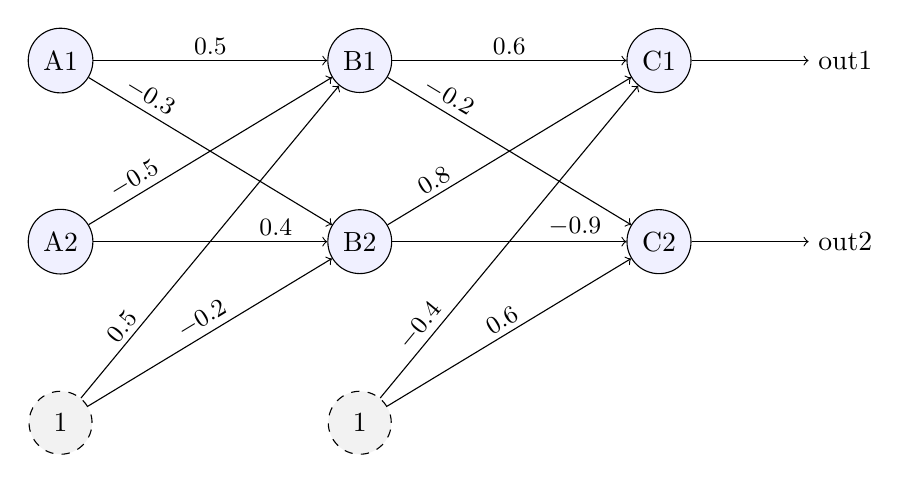
\begin{tikzpicture}[x=3.8cm,y=2.3cm,n/.style={circle,draw,minimum size=8mm,fill=blue!6},
  bn/.style={circle,draw,dashed,minimum size=8mm,fill=gray!10},
  w/.style={font=\small,fill=white,inner sep=1pt,sloped,above=1pt}]
\node[n] (A1) at (0,2) {A1}; \node[n] (A2) at (0,1) {A2}; \node[bn] (A0) at (0,0) {1};
\node[n] (B1) at (1,2) {B1}; \node[n] (B2) at (1,1) {B2}; \node[bn] (B0) at (1,0) {1};
\node[n] (C1) at (2,2) {C1}; \node[n] (C2) at (2,1) {C2};
% each weight is written near the start of its connection
\draw[->] (A1) -- node[w,pos=0.5] {0.5} (B1);
\draw[->] (A1) -- node[w,pos=0.22] {$-0.3$} (B2);
\draw[->] (A2) -- node[w,pos=0.22] {$-0.5$} (B1);
\draw[->] (A2) -- node[w,pos=0.78] {0.4} (B2);
\draw[->] (A0) -- node[w,pos=0.2] {0.5} (B1);
\draw[->] (A0) -- node[w,pos=0.5] {$-0.2$} (B2);
\draw[->] (B1) -- node[w,pos=0.5] {0.6} (C1);
\draw[->] (B1) -- node[w,pos=0.22] {$-0.2$} (C2);
\draw[->] (B2) -- node[w,pos=0.22] {0.8} (C1);
\draw[->] (B2) -- node[w,pos=0.78] {$-0.9$} (C2);
\draw[->] (B0) -- node[w,pos=0.2] {$-0.4$} (C1);
\draw[->] (B0) -- node[w,pos=0.5] {0.6} (C2);
\draw[->] (C1) -- ++(0.5,0) node[right] {out1}; \draw[->] (C2) -- ++(0.5,0) node[right] {out2};
\end{tikzpicture}
\end{center}
\prompt{Show the forward pass, in matrix form, of the record with Feature1 $= 4$ and Feature2 $= 2$. How would
this network classify the record (Class A or Class B)?}
\answerbox{10}
\begin{solution}
From the diagram:
\[
\bm{W}^{(1)} = \begin{pmatrix} 0.5 & -0.5 \\ -0.3 & 0.4 \end{pmatrix}, \quad
\bm{b}^{(1)} = \begin{pmatrix} 0.5 \\ -0.2 \end{pmatrix}, \quad
\bm{W}^{(2)} = \begin{pmatrix} 0.6 & 0.8 \\ -0.2 & -0.9 \end{pmatrix}, \quad
\bm{b}^{(2)} = \begin{pmatrix} -0.4 \\ 0.6 \end{pmatrix}.
\]
\[
\bm{z}_B = \bm{W}^{(1)} \bm{x} + \bm{b}^{(1)}
= \begin{pmatrix} 0.5 \cdot 4 - 0.5 \cdot 2 + 0.5 \\ -0.3 \cdot 4 + 0.4 \cdot 2 - 0.2 \end{pmatrix}
= \begin{pmatrix} 1.5 \\ -0.6 \end{pmatrix}, \quad
\bm{B} = \operatorname{ReLU}(\bm{z}_B) = \begin{pmatrix} 1.5 \\ 0 \end{pmatrix}
\]
\[
\bm{C} = \bm{W}^{(2)} \bm{B} + \bm{b}^{(2)}
= \begin{pmatrix} 0.6 \cdot 1.5 + 0.8 \cdot 0 - 0.4 \\ -0.2 \cdot 1.5 - 0.9 \cdot 0 + 0.6 \end{pmatrix}
= \begin{pmatrix} 0.5 \\ 0.3 \end{pmatrix}
\]
out1 $= 0.5 >$ out2 $= 0.3$: the network predicts Class A. (Forgetting the ReLU, and using
$B_2 = -0.6$, gives out1 $= 0.02$ and out2 $= 0.84$, the wrong class.)
\end{solution}

\newpage
\part[14] The network below has one hidden layer and one output, and will be trained for classification with log loss (cross-entropy loss). A record with inputs $A_1 = 2$,
$A_2 = 1$ and label $y = 1$ is passed in.
\begin{center}
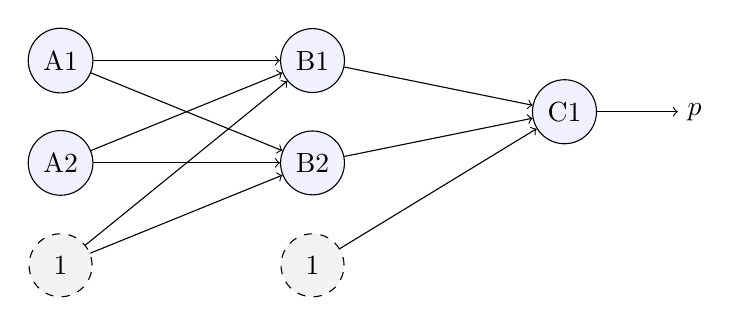
\begin{tikzpicture}[x=3.2cm,y=1.3cm,n/.style={circle,draw,minimum size=8mm,fill=blue!6},
  bn/.style={circle,draw,dashed,minimum size=8mm,fill=gray!10}]
\node[n] (A1) at (0,2) {A1}; \node[n] (A2) at (0,1) {A2}; \node[bn] (A0) at (0,0) {1};
\node[n] (B1) at (1,2) {B1}; \node[n] (B2) at (1,1) {B2}; \node[bn] (B0) at (1,0) {1};
\node[n] (C1) at (2,1.5) {C1};
\foreach \a in {A1,A2,A0} \foreach \b in {B1,B2} \draw[->] (\a) -- (\b);
\foreach \a in {B1,B2,B0} \draw[->] (\a) -- (C1);
\draw[->] (C1) -- ++(0.45,0) node[right] {$p$};
\end{tikzpicture}
\end{center}
\begin{center}
\begin{tabular}{|l|l|l|}
\hline
\rowcolor{headgray} activation function & function & derivative \\ \hline
B layer: sigmoid & $f(z) = 1/(1 + e^{-z})$ & $f(z)\,(1 - f(z))$ \\ \hline
C layer: sigmoid & $p = C_1 = 1/(1 + e^{-z_C})$ & (see the loss) \\ \hline
loss: cross-entropy & $\mathcal{L} = -y \log p - (1 - y) \log(1 - p)$ & $\partial \mathcal{L}/\partial z_C = p - y$ \\ \hline
\end{tabular}
\end{center}
Here $z_C$ is C1's input sum, and $p$ is the predicted probability that $y = 1$. The weights during the forward propagation are
\[
\bm{W}^{(1)} = \begin{pmatrix} 0.5 & -1.0 \\ 1.5 & 0.5 \end{pmatrix},\quad
\bm{b}^{(1)} = \begin{pmatrix} 0.5 \\ -1.0 \end{pmatrix},\qquad
\bm{W}^{(2)} = \begin{pmatrix} 1.0 & -2.0 \end{pmatrix},\quad b^{(2)} = 0.5 .
\]
You do not need to forward propagate. The node activations (output values) during the forward propagation are
\begin{center}
\begin{tabular}{|l|l|l|}
\hline
\rowcolor{headgray} A layer & B layer & C layer \\ \hline
$A_1 = 2$ & $B_1 = 0.62$ & $C_1 = p = 0.33$ \\ \hline
$A_2 = 1$ & $B_2 = 0.92$ & \\ \hline
\end{tabular}
\end{center}
Use a learning rate of 1. Compute every derivative with the weights above, the ones used in the
forward propagation.
\begin{subparts}
\subpart \prompt{Adjust $W^{(2)}_{11}$, the weight from B1 to C1.}
\answerbox[\thepartno(\thesubpart)]{5}
\ifprintanswers\else\newpage\fi   % keep (b) and its answer box together on the test
\subpart \prompt{Adjust $W^{(1)}_{11}$, the weight from A1 to B1.}
\answerbox[\thepartno(\thesubpart)]{10}
\end{subparts}
\begin{solution}
(a) The error at the output is $\partial \mathcal{L}/\partial z_C = p - y = 0.33 - 1 = -0.67$. Since
$z_C = W^{(2)}_{11} B_1 + W^{(2)}_{12} B_2 + b^{(2)}$, $\partial z_C/\partial W^{(2)}_{11} = B_1 = 0.62$, so
\[
\frac{\partial \mathcal{L}}{\partial W^{(2)}_{11}} = -0.67 \cdot 0.62 = -0.415, \qquad
W^{(2)}_{11} \leftarrow 1.0 - 1 \cdot (-0.415) = 1.415 .
\]
(b) The path is $W^{(1)}_{11} \to z_{B_1} \to B_1 \to z_C \to \mathcal{L}$, where $z_{B_1}$ is B1's input sum.
Reuse $-0.67$ from (a), with the old weight $W^{(2)}_{11} = 1.0$:
\[
\frac{\partial \mathcal{L}}{\partial B_1} = -0.67 \cdot 1.0 = -0.67, \qquad
\frac{\partial \mathcal{L}}{\partial z_{B_1}} = -0.67 \cdot B_1 (1 - B_1) = -0.67 \cdot 0.62 \cdot 0.38 = -0.158,
\]
\[
\frac{\partial \mathcal{L}}{\partial W^{(1)}_{11}} = -0.158 \cdot A_1 = -0.158 \cdot 2 = -0.316, \qquad
W^{(1)}_{11} \leftarrow 0.5 - 1 \cdot (-0.316) = 0.816 .
\]
(With unrounded node values the updates are 1.419 and 0.817; accept either.)
\end{solution}

\ifprintanswers\else\newpage\fi   % the short answers on one page of the test
\part Short answers (8 points in all).
\begin{subparts}
\subpart[3] \prompt{You train the same network twice with different learning rates and plot the training
loss after each epoch. In run 1 the loss jumps up and down and ends higher than it started. In run 2
it goes down steadily, but very slowly. For each run, is the learning rate too large or too small?
Why?}
\answerbox[\thepartno(\thesubpart)]{5}
\begin{solution}
Run 1: too large. Each step overshoots the minimum, so the loss bounces around and can grow.
Run 2: too small. Each step moves the weights only a little, so the loss falls slowly.
\end{solution}
\subpart[2] \prompt{A network classifies images into 3 classes. Why put a softmax on the three outputs
instead of a separate sigmoid on each?}
\answerbox[\thepartno(\thesubpart)]{4}
\begin{solution}
The softmax outputs are positive and add up to 1, so they are one probability distribution over the
3 classes. Separate sigmoids each give a number between 0 and 1, but they need not add up to 1 (all
three could be 0.9).
\end{solution}
\subpart[3] \prompt{A training set has 1,000 records. In one gradient-descent step, every weight in the
network is updated once. How many steps does training take in 5 epochs (number of passes through the
data) with (i) batch gradient descent, (ii) stochastic gradient descent (one record per step), and
(iii) mini-batches of 50 records?}
\answerbox[\thepartno(\thesubpart)]{4}
\begin{solution}
(i) One step per epoch: $5$. \quad (ii) $1{,}000$ steps per epoch: $5{,}000$. \quad
(iii) $1{,}000 / 50 = 20$ steps per epoch: $100$.
\end{solution}
\end{subparts}
\end{parts}

% ===================================================================== 5
\newpage
\titledquestion{Ensemble methods (10 points)}
\begin{parts}
\part[5] An SVM can only separate two classes. A clinic wants to classify chest X-rays into 4 classes:
normal, pneumonia, COVID and tuberculosis.
\begin{subparts}
\subpart \prompt{With one-vs-rest partitions, how many SVMs do you train, and what labels does each one
see?}
\subpart \prompt{How is a new X-ray classified?}
\subpart \prompt{With one-vs-one partitions, how many SVMs do you train?}
\end{subparts}
\answerbox{8}
\begin{solution}
(a) 4 SVMs, one per class. Each sees ``this class'' against ``the other three''.
(b) Each SVM predicts its side, and every class on the predicted side gets one vote; the class with the
most votes wins. (Also accept: pick the class whose SVM gives the largest $f(\bm{x})$.)
(c) One SVM for every pair of classes: $4 \cdot 3 / 2 = 6$.
\end{solution}

\part[3] \prompt{An ensemble of 25 classifiers is built, but each base classifier has error rate 0.6.
What happens to the error of the majority vote, compared with a single classifier? Why?}
\answerbox{5}
\begin{solution}
The ensemble is worse than a single classifier: with independent errors, the majority vote is wrong
whenever more than half of the classifiers are wrong, and with error 0.6 that happens most of the time
(about 0.85). A majority vote only helps when each base classifier is better than random guessing.
\end{solution}

\newpage
\part[2] \prompt{Random forests consider only a random subset of the features at each split. Why does
this help the ensemble?}
\answerbox{6}
\begin{solution}
It makes the trees less alike. Without it, every tree would split on the same strong features and make
similar mistakes; with random subsets the trees are more diverse, so their errors are less correlated
and the vote cancels more of them.
\end{solution}
\end{parts}

\end{questions}
\end{document}
"
\documentclass[11pt,addpoints]{exam}
\ifdefined\withsolutions \printanswers \fi
\usepackage{cs363m_exam}
\usepackage{pgfplots}
\pgfplotsset{compat=1.18}
\usepgfplotslibrary{groupplots}
% two options to circle: \pick{first}{second}{1 or 2}. The solutions circle the right one; the test
% draws the same frames invisibly, so the layout does not move.
\newcommand{\opt}[2]{% #2 is 1 for the right answer
  \def\optcolor{none}%
  \ifprintanswers\ifnum#2=1 \def\optcolor{red!70!black}\fi\fi
  \tikz[baseline=(o.base)]\node[inner sep=4pt,rounded corners=7pt,draw=\optcolor,very thick](o){#1};}
\newlength{\optw}\setlength{\optw}{3.6cm}   % each option sits in a column this wide
\newcommand{\pick}[3]{\hfill
  \makebox[\optw]{\ifnum#3=1 \opt{#1}{1}\else\opt{#1}{0}\fi}%
  \makebox[\optw]{\ifnum#3=2 \opt{#2}{1}\else\opt{#2}{0}\fi}}

\begin{document}
\ifprintanswers\examtitlepage{Midterm exam \textperiodcentered{} solutions}\else\examtitlepage{Midterm exam}\fi

\begin{questions}

% ===================================================================== 1
\titledquestion{Evaluating classifiers (20 points)}
A university wants to use an AI-text detector to check student essays. To test it, the detector is
run on 400 essays whose authorship is known: 60 were written with AI and 340 by students. Of the
400 essays, the detector flags 50 as written with AI. Of these 50 flagged essays, 45 really were
written with AI. Treat ``written with AI'' as the positive class.

\begin{parts}
\part[4] \prompt{Write down the confusion matrix.}
\ifprintanswers\else
\par\vspace{6pt}\noindent{\color{lbl}\textbf{Answer \thepartno}}
\begin{center}
\begin{tabular}{l|p{3cm}|p{3cm}|}
\multicolumn{1}{l}{} & \multicolumn{1}{c}{flagged} & \multicolumn{1}{c}{not flagged} \\
\cline{2-3}
written with AI & \rule[-0.45cm]{0pt}{1.2cm} & \\
\cline{2-3}
written by students & \rule[-0.45cm]{0pt}{1.2cm} & \\
\cline{2-3}
\end{tabular}
\end{center}
\fi
\begin{solution}
60 AI-written essays and 340 human-written essays.
\begin{center}
\begin{tabular}{|l|c|c|}
\hline
\rowcolor{headgray} & flagged & not flagged \\ \hline
written with AI & TP $= 45$ & FN $= 15$ \\ \hline
written by students & FP $= 5$  & TN $= 335$ \\ \hline
\end{tabular}
\end{center}
\end{solution}

\part[2] \prompt{What are precision and recall for this detector?}
\answerbox{5}
\begin{solution}
Precision $= 45/50 = 0.90$. \quad Recall $= 45/60 = 0.75$.
\end{solution}

\part[2] \prompt{Do we care more about improving precision or recall for this problem, and why?}
\answerbox{5}
\begin{solution}
Precision. A false positive accuses an innocent student of cheating; a missed AI essay (false
negative) is a smaller harm. A flag should almost always be right before anyone acts on it.
\end{solution}

\uplevel{The detector also gives each essay a score between 0 and 1; a higher score means ``more
likely written with AI''. Here are 8 essays, 4 written with AI and 4 by students:
\begin{center}
\begin{tabular}{|l|c|c|c|c|c|c|c|c|}
\hline
\rowcolor{headgray} essay            & 1 & 2 & 3 & 4 & 5 & 6 & 7 & 8 \\ \hline
score            & 0.95 & 0.85 & 0.70 & 0.60 & 0.50 & 0.40 & 0.30 & 0.10 \\ \hline
written with AI? & yes & yes & no & yes & no & yes & no & no \\ \hline
\end{tabular}
\end{center}
We say the detector flags an essay as AI-written if its score is over $t$.}

\part[10] \prompt{The ROC curve starts at $(\mathrm{FPR}, \mathrm{TPR}) = (0, 0)$, when $t$ is above every
score. Lower $t$ past one essay at a time. What are the next three points on the curve?}
\answerbox{8}
\begin{solution}
As $t$ passes each essay, from the highest score down, an AI essay moves the point up by
$1/4 = 0.25$ and a human essay moves it right by $0.25$. Essays 1 and 2 are AI-written and essay 3
is not, so the next three points are
\[
(0,\ 0.25), \quad (0,\ 0.5), \quad (0.25,\ 0.5).
\]
\end{solution}

\part[2] \prompt{Another detector has an AUC of 0.3 on the test essays. What does that tell you, and
what simple change would improve it?}
\answerbox{5}
\begin{solution}
It is worse than random guessing (AUC 0.5): it tends to give human-written essays higher scores than
AI-written ones. Flip it: use $1 - \text{score}$ (equivalently, flag the essays with low scores).
That reverses the order of the essays, so the AUC becomes $1 - 0.3 = 0.7$.
\end{solution}
\end{parts}

% ===================================================================== 2
\newpage
\titledquestion{Support vector machines (20 points)}
\begin{parts}
\part[10] A soft-margin SVM returned $\bm{w} = (6, 8)$, $b = -20$.
\begin{center}
\begin{tabular}{|l|c|c|c|}
\hline
\rowcolor{headgray} point  & C & D & E \\ \hline
$x_1$  & 1.5 & 1.25 & 3 \\ \hline
$x_2$  & 1.5 & 1.5 & 0.5 \\ \hline
label  & $+$ & $-$ & $-$ \\ \hline
\end{tabular}
\end{center}
\begin{subparts}
\subpart \prompt{Compute $f(\bm{x})$ and the predicted class of each point.}
\subpart \prompt{What is the width of the margin?}
\subpart \prompt{Which points are on the margin? Which points are inside the margin? Which points are
misclassified?}
\end{subparts}
\answerbox{16}
\begin{solution}
$f(\bm{x}) = 6x_1 + 8x_2 - 20$ and $\|\bm{w}\| = \sqrt{6^2 + 8^2} = 10$.
\begin{center}
\begin{tabular}{|l|c|c|c|}
\hline
\rowcolor{headgray} point & C & D & E \\ \hline
$f(\bm{x})$                       & $1$   & $-0.5$ & $2$ \\ \hline
predicted class                   & $+$   & $-$    & $+$ \\ \hline
$y\,f(\bm{x})$                    & $1$   & $0.5$  & $-2$ \\ \hline
\end{tabular}
\end{center}
(b) Margin width $= 2/\|\bm{w}\| = 2/10 = 0.2$.

(c) On the margin: C ($y\,f = 1$). Inside the margin: D ($0 < y\,f = 0.5 < 1$), still correctly
classified. Misclassified: E (label $-$, predicted $+$; $y\,f = -2$).
\end{solution}

\part[4] The soft-margin SVM solves
\[
\min_{\bm{w},\, b,\, \bm{\xi}} \ \tfrac12 \|\bm{w}\|^2 + C \sum_i \xi_i
\quad \text{subject to} \quad y_i(\bm{w} \cdot \bm{x}_i + b) \ge 1 - \xi_i,\ \ \xi_i \ge 0 .
\]
\begin{subparts}
\subpart \prompt{What does the slack $\xi_i$ measure, and why do we need it?}
\subpart \prompt{Where does a training point lie, relative to the margin and the decision boundary, if
$\xi_i > 1$?}
\end{subparts}
\answerbox{8}
\begin{solution}
(a) $\xi_i$ measures how far point $i$ falls short of being on its correct side, outside the margin.
Without slack, the constraints $y_i(\bm{w} \cdot \bm{x}_i + b) \ge 1$ have no solution when the
classes overlap; slack lets some points violate the margin, at a cost $C\xi_i$ each.

(b) On the wrong side of the decision boundary: misclassified. (At the solution
$\xi_i = \max(0,\, 1 - y_i f(\bm{x}_i))$, so $\xi_i > 1$ means $y_i f(\bm{x}_i) < 0$.)
\end{solution}

\part[4] Two soft-margin SVMs are trained on the same data, one with $C = 0.01$ and one with
$C = 100$.
For (a)--(c), circle one answer.
\begin{subparts}
\subpart \prompt{Which has the wider margin?} \pick{$C = 0.01$}{$C = 100$}{1}
\subpart \prompt{Which has more support vectors?} \pick{$C = 0.01$}{$C = 100$}{1}
\subpart \prompt{Which is more likely to overfit?} \pick{$C = 0.01$}{$C = 100$}{2}
\subpart \prompt{How would you choose $C$ in practice, and why?}
\end{subparts}
\answerbox[\thepartno(d)]{4}
\begin{solution}
(a) $C = 0.01$: slack is cheap, so the SVM accepts many points inside the margin in exchange for a
wider one.
(b) $C = 0.01$: with a wider margin, more points fall on or inside it, and all of them are support
vectors.
(c) $C = 100$: violations are expensive, so the margin narrows to fit individual training points.
(d) $C$ is a hyperparameter: try several values and pick the one with the best accuracy on
validation data (or by cross-validation). Training accuracy cannot choose it, because a larger $C$
always fits the training data at least as well; only held-out data shows which $C$ generalizes.
\end{solution}

\ifprintanswers\else\newpage\fi   % keep 2.4 together on the test
\part[2] \prompt{You remove a training point that is not a support vector and retrain the SVM. What
changes? Why?}
\answerbox{5}
\begin{solution}
Nothing. The solution depends only on the support vectors; a point outside the margin does not
affect $\bm{w}$ or $b$.
\end{solution}
\end{parts}

% ===================================================================== 3
\newpage
\titledquestion{Nonlinear regression (20 points)}
\begin{parts}
\part[4] kNN regression is trained on six points:
\begin{center}
\begin{tabular}{|l|c|c|c|c|c|c|}
\hline
$x$ & 1 & 2 & 4 & 5 & 7 & 8 \\ \hline
$y$ & 3 & 6 & 4 & 8 & 10 & 12 \\ \hline
\end{tabular}
\end{center}
\prompt{Predict $y$ at $x = 4.4$ using (a) $k = 1$ and (b) $k = 3$.}
\answerbox{3}
\begin{solution}
(a) The nearest point is $x = 4$, so the prediction is $4$.
(b) The three nearest points are $x = 4, 5, 2$ (distances $0.4, 0.6, 2.4$), so the prediction is
$(4 + 8 + 6)/3 = 6$.
\end{solution}

\part[6] \prompt{For each model, name a hyperparameter that controls how closely the model fits the
training data. Does increasing it make overfitting more likely or less likely? Fill in the table.}
\begin{center}
\renewcommand{\arraystretch}{1.25}
\ifprintanswers
\begin{tabular}{|>{\raggedright\arraybackslash}p{3.3cm}|>{\raggedright\arraybackslash}p{5.2cm}|>{\raggedright\arraybackslash}p{4.2cm}|}
\hline
\rowcolor{headgray} \textbf{Model} & \textbf{Hyperparameter} & \textbf{Increasing it $\to$}\newline \textbf{MORE / LESS overfitting} \\ \hline
Regression tree & maximum depth & MORE \\ \hline
kNN regression & number of neighbours $k$ & LESS \\ \hline
SVR & $C$ & MORE \\ \hline
\end{tabular}
\else
\begin{tabular}{|>{\raggedright\arraybackslash}p{3.3cm}|>{\raggedright\arraybackslash}p{5.2cm}|>{\raggedright\arraybackslash}p{4.2cm}|}
\hline
\rowcolor{headgray} \textbf{Model} & \textbf{Hyperparameter} & \textbf{Increasing it $\to$}\newline \textbf{MORE / LESS overfitting} \\ \hline
Regression tree \rule[-0.5cm]{0pt}{1.3cm} & & \\ \hline
kNN regression \rule[-0.5cm]{0pt}{1.3cm} & & \\ \hline
SVR \rule[-0.5cm]{0pt}{1.3cm} & & \\ \hline
\end{tabular}
\fi
\end{center}
\begin{solution}
Other correct answers: for the tree, the minimum number of points needed to split (increasing it:
LESS); for SVR, $\varepsilon$ (increasing it: LESS). The direction must match the hyperparameter named.
\end{solution}

\newpage
\part[5] \prompt{The figure shows three models fitted to the same data. Which panel shows a regression
tree, which shows kNN with $k = 1$, and which shows SVR with a kernel? Explain each.}
\begin{center}
% Question 3.3 of the exam: three fits of the same data (data from ../make_figure.py)
\begin{tikzpicture}
\begin{groupplot}[group style={group size=3 by 1, horizontal sep=1.1cm},
    width=5.6cm, height=4.6cm, xmin=0, xmax=10, ymin=2.5, ymax=7, xtick={0,5,10}, ytick={3,5,7},
    xlabel={$x$}, ylabel={$y$}, ylabel style={yshift=-4pt}, title style={font=\bfseries}]
\nextgroupplot[title=A]
  \addplot[thick, blue!70!black] table {fig_data/svr.dat};
  \addplot[only marks, mark=*, mark size=1.6pt] table {fig_data/points.dat};
\nextgroupplot[title=B]
  \addplot[thick, blue!70!black] table {fig_data/tree.dat};
  \addplot[only marks, mark=*, mark size=1.6pt] table {fig_data/points.dat};
\nextgroupplot[title=C]
  \addplot[thick, blue!70!black] table {fig_data/knn.dat};
  \addplot[only marks, mark=*, mark size=1.6pt] table {fig_data/points.dat};
\end{groupplot}
\end{tikzpicture}

\end{center}
\answerbox{6}
\begin{solution}
A is SVR with a kernel: a smooth curve. B is the regression tree: a few wide flat steps, one for
each leaf, which predicts the average $y$ of its points. C is kNN with $k = 1$: a narrow step for
every training point, passing through every point.
\end{solution}

\part[5] \prompt{Suppose you use kNN to predict house prices from floor area (500 to 5,000 square feet) and number
of bedrooms (1 to 6). Why might kNN do badly on these raw features? What would you do?}
\answerbox{6}
\begin{solution}
Distances are dominated by floor area: a difference of one bedroom counts as much as one square
foot, so the nearest houses match on area and almost ignore bedrooms. Standardize each feature
(subtract its mean, divide by its standard deviation) before computing distances.
\end{solution}
\end{parts}

% ===================================================================== 4
\newpage
\titledquestion{Neural networks (30 points)}
In this question, row $j$ of a weight matrix $\bm{W}^{(l)}$ holds the weights into node $j$ of layer
$l$: $W^{(l)}_{ji}$ is the weight from node $i$ of the previous layer to node $j$. The bias of node
$j$ is $b^{(l)}_j$, the weight on the input that is always 1.

\begin{parts}
\part[8] In the network below, out1 represents Class A and out2 represents Class B. The hidden nodes
B1 and B2 use the ReLU activation, $\operatorname{ReLU}(z) = \max(0, z)$. The output nodes C1 and C2
have no activation: each outputs its weighted sum. The network predicts the class whose output is
larger.
\begin{center}
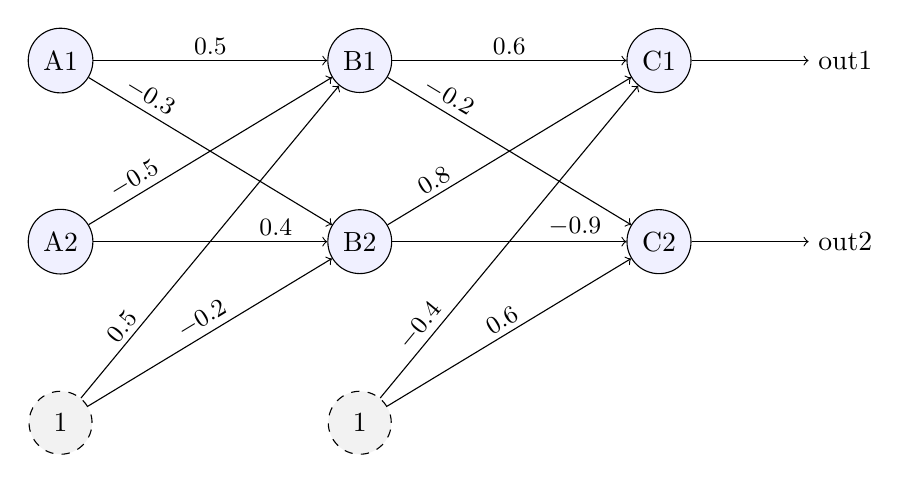
\begin{tikzpicture}[x=3.8cm,y=2.3cm,n/.style={circle,draw,minimum size=8mm,fill=blue!6},
  bn/.style={circle,draw,dashed,minimum size=8mm,fill=gray!10},
  w/.style={font=\small,fill=white,inner sep=1pt,sloped,above=1pt}]
\node[n] (A1) at (0,2) {A1}; \node[n] (A2) at (0,1) {A2}; \node[bn] (A0) at (0,0) {1};
\node[n] (B1) at (1,2) {B1}; \node[n] (B2) at (1,1) {B2}; \node[bn] (B0) at (1,0) {1};
\node[n] (C1) at (2,2) {C1}; \node[n] (C2) at (2,1) {C2};
% each weight is written near the start of its connection
\draw[->] (A1) -- node[w,pos=0.5] {0.5} (B1);
\draw[->] (A1) -- node[w,pos=0.22] {$-0.3$} (B2);
\draw[->] (A2) -- node[w,pos=0.22] {$-0.5$} (B1);
\draw[->] (A2) -- node[w,pos=0.78] {0.4} (B2);
\draw[->] (A0) -- node[w,pos=0.2] {0.5} (B1);
\draw[->] (A0) -- node[w,pos=0.5] {$-0.2$} (B2);
\draw[->] (B1) -- node[w,pos=0.5] {0.6} (C1);
\draw[->] (B1) -- node[w,pos=0.22] {$-0.2$} (C2);
\draw[->] (B2) -- node[w,pos=0.22] {0.8} (C1);
\draw[->] (B2) -- node[w,pos=0.78] {$-0.9$} (C2);
\draw[->] (B0) -- node[w,pos=0.2] {$-0.4$} (C1);
\draw[->] (B0) -- node[w,pos=0.5] {0.6} (C2);
\draw[->] (C1) -- ++(0.5,0) node[right] {out1}; \draw[->] (C2) -- ++(0.5,0) node[right] {out2};
\end{tikzpicture}
\end{center}
\prompt{Show the forward pass, in matrix form, of the record with Feature1 $= 4$ and Feature2 $= 2$. How would
this network classify the record (Class A or Class B)?}
\answerbox{10}
\begin{solution}
From the diagram:
\[
\bm{W}^{(1)} = \begin{pmatrix} 0.5 & -0.5 \\ -0.3 & 0.4 \end{pmatrix}, \quad
\bm{b}^{(1)} = \begin{pmatrix} 0.5 \\ -0.2 \end{pmatrix}, \quad
\bm{W}^{(2)} = \begin{pmatrix} 0.6 & 0.8 \\ -0.2 & -0.9 \end{pmatrix}, \quad
\bm{b}^{(2)} = \begin{pmatrix} -0.4 \\ 0.6 \end{pmatrix}.
\]
\[
\bm{z}_B = \bm{W}^{(1)} \bm{x} + \bm{b}^{(1)}
= \begin{pmatrix} 0.5 \cdot 4 - 0.5 \cdot 2 + 0.5 \\ -0.3 \cdot 4 + 0.4 \cdot 2 - 0.2 \end{pmatrix}
= \begin{pmatrix} 1.5 \\ -0.6 \end{pmatrix}, \quad
\bm{B} = \operatorname{ReLU}(\bm{z}_B) = \begin{pmatrix} 1.5 \\ 0 \end{pmatrix}
\]
\[
\bm{C} = \bm{W}^{(2)} \bm{B} + \bm{b}^{(2)}
= \begin{pmatrix} 0.6 \cdot 1.5 + 0.8 \cdot 0 - 0.4 \\ -0.2 \cdot 1.5 - 0.9 \cdot 0 + 0.6 \end{pmatrix}
= \begin{pmatrix} 0.5 \\ 0.3 \end{pmatrix}
\]
out1 $= 0.5 >$ out2 $= 0.3$: the network predicts Class A. (Forgetting the ReLU, and using
$B_2 = -0.6$, gives out1 $= 0.02$ and out2 $= 0.84$, the wrong class.)
\end{solution}

\newpage
\part[14] The network below has one hidden layer and one output, and will be trained for classification with log loss (cross-entropy loss). A record with inputs $A_1 = 2$,
$A_2 = 1$ and label $y = 1$ is passed in.
\begin{center}
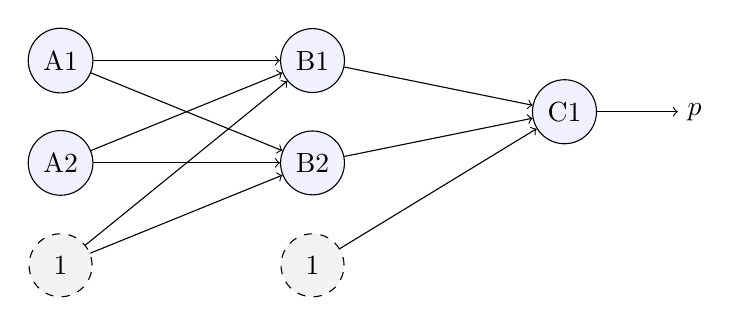
\begin{tikzpicture}[x=3.2cm,y=1.3cm,n/.style={circle,draw,minimum size=8mm,fill=blue!6},
  bn/.style={circle,draw,dashed,minimum size=8mm,fill=gray!10}]
\node[n] (A1) at (0,2) {A1}; \node[n] (A2) at (0,1) {A2}; \node[bn] (A0) at (0,0) {1};
\node[n] (B1) at (1,2) {B1}; \node[n] (B2) at (1,1) {B2}; \node[bn] (B0) at (1,0) {1};
\node[n] (C1) at (2,1.5) {C1};
\foreach \a in {A1,A2,A0} \foreach \b in {B1,B2} \draw[->] (\a) -- (\b);
\foreach \a in {B1,B2,B0} \draw[->] (\a) -- (C1);
\draw[->] (C1) -- ++(0.45,0) node[right] {$p$};
\end{tikzpicture}
\end{center}
\begin{center}
\begin{tabular}{|l|l|l|}
\hline
\rowcolor{headgray} activation function & function & derivative \\ \hline
B layer: sigmoid & $f(z) = 1/(1 + e^{-z})$ & $f(z)\,(1 - f(z))$ \\ \hline
C layer: sigmoid & $p = C_1 = 1/(1 + e^{-z_C})$ & (see the loss) \\ \hline
loss: cross-entropy & $\mathcal{L} = -y \log p - (1 - y) \log(1 - p)$ & $\partial \mathcal{L}/\partial z_C = p - y$ \\ \hline
\end{tabular}
\end{center}
Here $z_C$ is C1's input sum, and $p$ is the predicted probability that $y = 1$. The weights during the forward propagation are
\[
\bm{W}^{(1)} = \begin{pmatrix} 0.5 & -1.0 \\ 1.5 & 0.5 \end{pmatrix},\quad
\bm{b}^{(1)} = \begin{pmatrix} 0.5 \\ -1.0 \end{pmatrix},\qquad
\bm{W}^{(2)} = \begin{pmatrix} 1.0 & -2.0 \end{pmatrix},\quad b^{(2)} = 0.5 .
\]
You do not need to forward propagate. The node activations (output values) during the forward propagation are
\begin{center}
\begin{tabular}{|l|l|l|}
\hline
\rowcolor{headgray} A layer & B layer & C layer \\ \hline
$A_1 = 2$ & $B_1 = 0.62$ & $C_1 = p = 0.33$ \\ \hline
$A_2 = 1$ & $B_2 = 0.92$ & \\ \hline
\end{tabular}
\end{center}
Use a learning rate of 1. Compute every derivative with the weights above, the ones used in the
forward propagation.
\begin{subparts}
\subpart \prompt{Adjust $W^{(2)}_{11}$, the weight from B1 to C1.}
\answerbox[\thepartno(\thesubpart)]{5}
\ifprintanswers\else\newpage\fi   % keep (b) and its answer box together on the test
\subpart \prompt{Adjust $W^{(1)}_{11}$, the weight from A1 to B1.}
\answerbox[\thepartno(\thesubpart)]{10}
\end{subparts}
\begin{solution}
(a) The error at the output is $\partial \mathcal{L}/\partial z_C = p - y = 0.33 - 1 = -0.67$. Since
$z_C = W^{(2)}_{11} B_1 + W^{(2)}_{12} B_2 + b^{(2)}$, $\partial z_C/\partial W^{(2)}_{11} = B_1 = 0.62$, so
\[
\frac{\partial \mathcal{L}}{\partial W^{(2)}_{11}} = -0.67 \cdot 0.62 = -0.415, \qquad
W^{(2)}_{11} \leftarrow 1.0 - 1 \cdot (-0.415) = 1.415 .
\]
(b) The path is $W^{(1)}_{11} \to z_{B_1} \to B_1 \to z_C \to \mathcal{L}$, where $z_{B_1}$ is B1's input sum.
Reuse $-0.67$ from (a), with the old weight $W^{(2)}_{11} = 1.0$:
\[
\frac{\partial \mathcal{L}}{\partial B_1} = -0.67 \cdot 1.0 = -0.67, \qquad
\frac{\partial \mathcal{L}}{\partial z_{B_1}} = -0.67 \cdot B_1 (1 - B_1) = -0.67 \cdot 0.62 \cdot 0.38 = -0.158,
\]
\[
\frac{\partial \mathcal{L}}{\partial W^{(1)}_{11}} = -0.158 \cdot A_1 = -0.158 \cdot 2 = -0.316, \qquad
W^{(1)}_{11} \leftarrow 0.5 - 1 \cdot (-0.316) = 0.816 .
\]
(With unrounded node values the updates are 1.419 and 0.817; accept either.)
\end{solution}

\ifprintanswers\else\newpage\fi   % the short answers on one page of the test
\part Short answers (8 points in all).
\begin{subparts}
\subpart[3] \prompt{You train the same network twice with different learning rates and plot the training
loss after each epoch. In run 1 the loss jumps up and down and ends higher than it started. In run 2
it goes down steadily, but very slowly. For each run, is the learning rate too large or too small?
Why?}
\answerbox[\thepartno(\thesubpart)]{5}
\begin{solution}
Run 1: too large. Each step overshoots the minimum, so the loss bounces around and can grow.
Run 2: too small. Each step moves the weights only a little, so the loss falls slowly.
\end{solution}
\subpart[2] \prompt{A network classifies images into 3 classes. Why put a softmax on the three outputs
instead of a separate sigmoid on each?}
\answerbox[\thepartno(\thesubpart)]{4}
\begin{solution}
The softmax outputs are positive and add up to 1, so they are one probability distribution over the
3 classes. Separate sigmoids each give a number between 0 and 1, but they need not add up to 1 (all
three could be 0.9).
\end{solution}
\subpart[3] \prompt{A training set has 1,000 records. In one gradient-descent step, every weight in the
network is updated once. How many steps does training take in 5 epochs (number of passes through the
data) with (i) batch gradient descent, (ii) stochastic gradient descent (one record per step), and
(iii) mini-batches of 50 records?}
\answerbox[\thepartno(\thesubpart)]{4}
\begin{solution}
(i) One step per epoch: $5$. \quad (ii) $1{,}000$ steps per epoch: $5{,}000$. \quad
(iii) $1{,}000 / 50 = 20$ steps per epoch: $100$.
\end{solution}
\end{subparts}
\end{parts}

% ===================================================================== 5
\newpage
\titledquestion{Ensemble methods (10 points)}
\begin{parts}
\part[5] An SVM can only separate two classes. A clinic wants to classify chest X-rays into 4 classes:
normal, pneumonia, COVID and tuberculosis.
\begin{subparts}
\subpart \prompt{With one-vs-rest partitions, how many SVMs do you train, and what labels does each one
see?}
\subpart \prompt{How is a new X-ray classified?}
\subpart \prompt{With one-vs-one partitions, how many SVMs do you train?}
\end{subparts}
\answerbox{8}
\begin{solution}
(a) 4 SVMs, one per class. Each sees ``this class'' against ``the other three''.
(b) Each SVM predicts its side, and every class on the predicted side gets one vote; the class with the
most votes wins. (Also accept: pick the class whose SVM gives the largest $f(\bm{x})$.)
(c) One SVM for every pair of classes: $4 \cdot 3 / 2 = 6$.
\end{solution}

\part[3] \prompt{An ensemble of 25 classifiers is built, but each base classifier has error rate 0.6.
What happens to the error of the majority vote, compared with a single classifier? Why?}
\answerbox{5}
\begin{solution}
The ensemble is worse than a single classifier: with independent errors, the majority vote is wrong
whenever more than half of the classifiers are wrong, and with error 0.6 that happens most of the time
(about 0.85). A majority vote only helps when each base classifier is better than random guessing.
\end{solution}

\newpage
\part[2] \prompt{Random forests consider only a random subset of the features at each split. Why does
this help the ensemble?}
\answerbox{6}
\begin{solution}
It makes the trees less alike. Without it, every tree would split on the same strong features and make
similar mistakes; with random subsets the trees are more diverse, so their errors are less correlated
and the vote cancels more of them.
\end{solution}
\end{parts}

\end{questions}
\end{document}
"
\documentclass[11pt,addpoints]{exam}
\ifdefined\withsolutions \printanswers \fi
\usepackage{cs363m_exam}
\usepackage{pgfplots}
\pgfplotsset{compat=1.18}
\usepgfplotslibrary{groupplots}
% two options to circle: \pick{first}{second}{1 or 2}. The solutions circle the right one; the test
% draws the same frames invisibly, so the layout does not move.
\newcommand{\opt}[2]{% #2 is 1 for the right answer
  \def\optcolor{none}%
  \ifprintanswers\ifnum#2=1 \def\optcolor{red!70!black}\fi\fi
  \tikz[baseline=(o.base)]\node[inner sep=4pt,rounded corners=7pt,draw=\optcolor,very thick](o){#1};}
\newlength{\optw}\setlength{\optw}{3.6cm}   % each option sits in a column this wide
\newcommand{\pick}[3]{\hfill
  \makebox[\optw]{\ifnum#3=1 \opt{#1}{1}\else\opt{#1}{0}\fi}%
  \makebox[\optw]{\ifnum#3=2 \opt{#2}{1}\else\opt{#2}{0}\fi}}

\begin{document}
\ifprintanswers\examtitlepage{Midterm exam \textperiodcentered{} solutions}\else\examtitlepage{Midterm exam}\fi

\begin{questions}

% ===================================================================== 1
\titledquestion{Evaluating classifiers (20 points)}
A university wants to use an AI-text detector to check student essays. To test it, the detector is
run on 400 essays whose authorship is known: 60 were written with AI and 340 by students. Of the
400 essays, the detector flags 50 as written with AI. Of these 50 flagged essays, 45 really were
written with AI. Treat ``written with AI'' as the positive class.

\begin{parts}
\part[4] \prompt{Write down the confusion matrix.}
\ifprintanswers\else
\par\vspace{6pt}\noindent{\color{lbl}\textbf{Answer \thepartno}}
\begin{center}
\begin{tabular}{l|p{3cm}|p{3cm}|}
\multicolumn{1}{l}{} & \multicolumn{1}{c}{flagged} & \multicolumn{1}{c}{not flagged} \\
\cline{2-3}
written with AI & \rule[-0.45cm]{0pt}{1.2cm} & \\
\cline{2-3}
written by students & \rule[-0.45cm]{0pt}{1.2cm} & \\
\cline{2-3}
\end{tabular}
\end{center}
\fi
\begin{solution}
60 AI-written essays and 340 human-written essays.
\begin{center}
\begin{tabular}{|l|c|c|}
\hline
\rowcolor{headgray} & flagged & not flagged \\ \hline
written with AI & TP $= 45$ & FN $= 15$ \\ \hline
written by students & FP $= 5$  & TN $= 335$ \\ \hline
\end{tabular}
\end{center}
\end{solution}

\part[2] \prompt{What are precision and recall for this detector?}
\answerbox{5}
\begin{solution}
Precision $= 45/50 = 0.90$. \quad Recall $= 45/60 = 0.75$.
\end{solution}

\part[2] \prompt{Do we care more about improving precision or recall for this problem, and why?}
\answerbox{5}
\begin{solution}
Precision. A false positive accuses an innocent student of cheating; a missed AI essay (false
negative) is a smaller harm. A flag should almost always be right before anyone acts on it.
\end{solution}

\uplevel{The detector also gives each essay a score between 0 and 1; a higher score means ``more
likely written with AI''. Here are 8 essays, 4 written with AI and 4 by students:
\begin{center}
\begin{tabular}{|l|c|c|c|c|c|c|c|c|}
\hline
\rowcolor{headgray} essay            & 1 & 2 & 3 & 4 & 5 & 6 & 7 & 8 \\ \hline
score            & 0.95 & 0.85 & 0.70 & 0.60 & 0.50 & 0.40 & 0.30 & 0.10 \\ \hline
written with AI? & yes & yes & no & yes & no & yes & no & no \\ \hline
\end{tabular}
\end{center}
We say the detector flags an essay as AI-written if its score is over $t$.}

\part[10] \prompt{The ROC curve starts at $(\mathrm{FPR}, \mathrm{TPR}) = (0, 0)$, when $t$ is above every
score. Lower $t$ past one essay at a time. What are the next three points on the curve?}
\answerbox{8}
\begin{solution}
As $t$ passes each essay, from the highest score down, an AI essay moves the point up by
$1/4 = 0.25$ and a human essay moves it right by $0.25$. Essays 1 and 2 are AI-written and essay 3
is not, so the next three points are
\[
(0,\ 0.25), \quad (0,\ 0.5), \quad (0.25,\ 0.5).
\]
\end{solution}

\part[2] \prompt{Another detector has an AUC of 0.3 on the test essays. What does that tell you, and
what simple change would improve it?}
\answerbox{5}
\begin{solution}
It is worse than random guessing (AUC 0.5): it tends to give human-written essays higher scores than
AI-written ones. Flip it: use $1 - \text{score}$ (equivalently, flag the essays with low scores).
That reverses the order of the essays, so the AUC becomes $1 - 0.3 = 0.7$.
\end{solution}
\end{parts}

% ===================================================================== 2
\newpage
\titledquestion{Support vector machines (20 points)}
\begin{parts}
\part[10] A soft-margin SVM returned $\bm{w} = (6, 8)$, $b = -20$.
\begin{center}
\begin{tabular}{|l|c|c|c|}
\hline
\rowcolor{headgray} point  & C & D & E \\ \hline
$x_1$  & 1.5 & 1.25 & 3 \\ \hline
$x_2$  & 1.5 & 1.5 & 0.5 \\ \hline
label  & $+$ & $-$ & $-$ \\ \hline
\end{tabular}
\end{center}
\begin{subparts}
\subpart \prompt{Compute $f(\bm{x})$ and the predicted class of each point.}
\subpart \prompt{What is the width of the margin?}
\subpart \prompt{Which points are on the margin? Which points are inside the margin? Which points are
misclassified?}
\end{subparts}
\answerbox{16}
\begin{solution}
$f(\bm{x}) = 6x_1 + 8x_2 - 20$ and $\|\bm{w}\| = \sqrt{6^2 + 8^2} = 10$.
\begin{center}
\begin{tabular}{|l|c|c|c|}
\hline
\rowcolor{headgray} point & C & D & E \\ \hline
$f(\bm{x})$                       & $1$   & $-0.5$ & $2$ \\ \hline
predicted class                   & $+$   & $-$    & $+$ \\ \hline
$y\,f(\bm{x})$                    & $1$   & $0.5$  & $-2$ \\ \hline
\end{tabular}
\end{center}
(b) Margin width $= 2/\|\bm{w}\| = 2/10 = 0.2$.

(c) On the margin: C ($y\,f = 1$). Inside the margin: D ($0 < y\,f = 0.5 < 1$), still correctly
classified. Misclassified: E (label $-$, predicted $+$; $y\,f = -2$).
\end{solution}

\part[4] The soft-margin SVM solves
\[
\min_{\bm{w},\, b,\, \bm{\xi}} \ \tfrac12 \|\bm{w}\|^2 + C \sum_i \xi_i
\quad \text{subject to} \quad y_i(\bm{w} \cdot \bm{x}_i + b) \ge 1 - \xi_i,\ \ \xi_i \ge 0 .
\]
\begin{subparts}
\subpart \prompt{What does the slack $\xi_i$ measure, and why do we need it?}
\subpart \prompt{Where does a training point lie, relative to the margin and the decision boundary, if
$\xi_i > 1$?}
\end{subparts}
\answerbox{8}
\begin{solution}
(a) $\xi_i$ measures how far point $i$ falls short of being on its correct side, outside the margin.
Without slack, the constraints $y_i(\bm{w} \cdot \bm{x}_i + b) \ge 1$ have no solution when the
classes overlap; slack lets some points violate the margin, at a cost $C\xi_i$ each.

(b) On the wrong side of the decision boundary: misclassified. (At the solution
$\xi_i = \max(0,\, 1 - y_i f(\bm{x}_i))$, so $\xi_i > 1$ means $y_i f(\bm{x}_i) < 0$.)
\end{solution}

\part[4] Two soft-margin SVMs are trained on the same data, one with $C = 0.01$ and one with
$C = 100$.
For (a)--(c), circle one answer.
\begin{subparts}
\subpart \prompt{Which has the wider margin?} \pick{$C = 0.01$}{$C = 100$}{1}
\subpart \prompt{Which has more support vectors?} \pick{$C = 0.01$}{$C = 100$}{1}
\subpart \prompt{Which is more likely to overfit?} \pick{$C = 0.01$}{$C = 100$}{2}
\subpart \prompt{How would you choose $C$ in practice, and why?}
\end{subparts}
\answerbox[\thepartno(d)]{4}
\begin{solution}
(a) $C = 0.01$: slack is cheap, so the SVM accepts many points inside the margin in exchange for a
wider one.
(b) $C = 0.01$: with a wider margin, more points fall on or inside it, and all of them are support
vectors.
(c) $C = 100$: violations are expensive, so the margin narrows to fit individual training points.
(d) $C$ is a hyperparameter: try several values and pick the one with the best accuracy on
validation data (or by cross-validation). Training accuracy cannot choose it, because a larger $C$
always fits the training data at least as well; only held-out data shows which $C$ generalizes.
\end{solution}

\ifprintanswers\else\newpage\fi   % keep 2.4 together on the test
\part[2] \prompt{You remove a training point that is not a support vector and retrain the SVM. What
changes? Why?}
\answerbox{5}
\begin{solution}
Nothing. The solution depends only on the support vectors; a point outside the margin does not
affect $\bm{w}$ or $b$.
\end{solution}
\end{parts}

% ===================================================================== 3
\newpage
\titledquestion{Nonlinear regression (20 points)}
\begin{parts}
\part[4] kNN regression is trained on six points:
\begin{center}
\begin{tabular}{|l|c|c|c|c|c|c|}
\hline
$x$ & 1 & 2 & 4 & 5 & 7 & 8 \\ \hline
$y$ & 3 & 6 & 4 & 8 & 10 & 12 \\ \hline
\end{tabular}
\end{center}
\prompt{Predict $y$ at $x = 4.4$ using (a) $k = 1$ and (b) $k = 3$.}
\answerbox{3}
\begin{solution}
(a) The nearest point is $x = 4$, so the prediction is $4$.
(b) The three nearest points are $x = 4, 5, 2$ (distances $0.4, 0.6, 2.4$), so the prediction is
$(4 + 8 + 6)/3 = 6$.
\end{solution}

\part[6] \prompt{For each model, name a hyperparameter that controls how closely the model fits the
training data. Does increasing it make overfitting more likely or less likely? Fill in the table.}
\begin{center}
\renewcommand{\arraystretch}{1.25}
\ifprintanswers
\begin{tabular}{|>{\raggedright\arraybackslash}p{3.3cm}|>{\raggedright\arraybackslash}p{5.2cm}|>{\raggedright\arraybackslash}p{4.2cm}|}
\hline
\rowcolor{headgray} \textbf{Model} & \textbf{Hyperparameter} & \textbf{Increasing it $\to$}\newline \textbf{MORE / LESS overfitting} \\ \hline
Regression tree & maximum depth & MORE \\ \hline
kNN regression & number of neighbours $k$ & LESS \\ \hline
SVR & $C$ & MORE \\ \hline
\end{tabular}
\else
\begin{tabular}{|>{\raggedright\arraybackslash}p{3.3cm}|>{\raggedright\arraybackslash}p{5.2cm}|>{\raggedright\arraybackslash}p{4.2cm}|}
\hline
\rowcolor{headgray} \textbf{Model} & \textbf{Hyperparameter} & \textbf{Increasing it $\to$}\newline \textbf{MORE / LESS overfitting} \\ \hline
Regression tree \rule[-0.5cm]{0pt}{1.3cm} & & \\ \hline
kNN regression \rule[-0.5cm]{0pt}{1.3cm} & & \\ \hline
SVR \rule[-0.5cm]{0pt}{1.3cm} & & \\ \hline
\end{tabular}
\fi
\end{center}
\begin{solution}
Other correct answers: for the tree, the minimum number of points needed to split (increasing it:
LESS); for SVR, $\varepsilon$ (increasing it: LESS). The direction must match the hyperparameter named.
\end{solution}

\newpage
\part[5] \prompt{The figure shows three models fitted to the same data. Which panel shows a regression
tree, which shows kNN with $k = 1$, and which shows SVR with a kernel? Explain each.}
\begin{center}
% Question 3.3 of the exam: three fits of the same data (data from ../make_figure.py)
\begin{tikzpicture}
\begin{groupplot}[group style={group size=3 by 1, horizontal sep=1.1cm},
    width=5.6cm, height=4.6cm, xmin=0, xmax=10, ymin=2.5, ymax=7, xtick={0,5,10}, ytick={3,5,7},
    xlabel={$x$}, ylabel={$y$}, ylabel style={yshift=-4pt}, title style={font=\bfseries}]
\nextgroupplot[title=A]
  \addplot[thick, blue!70!black] table {fig_data/svr.dat};
  \addplot[only marks, mark=*, mark size=1.6pt] table {fig_data/points.dat};
\nextgroupplot[title=B]
  \addplot[thick, blue!70!black] table {fig_data/tree.dat};
  \addplot[only marks, mark=*, mark size=1.6pt] table {fig_data/points.dat};
\nextgroupplot[title=C]
  \addplot[thick, blue!70!black] table {fig_data/knn.dat};
  \addplot[only marks, mark=*, mark size=1.6pt] table {fig_data/points.dat};
\end{groupplot}
\end{tikzpicture}

\end{center}
\answerbox{6}
\begin{solution}
A is SVR with a kernel: a smooth curve. B is the regression tree: a few wide flat steps, one for
each leaf, which predicts the average $y$ of its points. C is kNN with $k = 1$: a narrow step for
every training point, passing through every point.
\end{solution}

\part[5] \prompt{Suppose you use kNN to predict house prices from floor area (500 to 5,000 square feet) and number
of bedrooms (1 to 6). Why might kNN do badly on these raw features? What would you do?}
\answerbox{6}
\begin{solution}
Distances are dominated by floor area: a difference of one bedroom counts as much as one square
foot, so the nearest houses match on area and almost ignore bedrooms. Standardize each feature
(subtract its mean, divide by its standard deviation) before computing distances.
\end{solution}
\end{parts}

% ===================================================================== 4
\newpage
\titledquestion{Neural networks (30 points)}
In this question, row $j$ of a weight matrix $\bm{W}^{(l)}$ holds the weights into node $j$ of layer
$l$: $W^{(l)}_{ji}$ is the weight from node $i$ of the previous layer to node $j$. The bias of node
$j$ is $b^{(l)}_j$, the weight on the input that is always 1.

\begin{parts}
\part[8] In the network below, out1 represents Class A and out2 represents Class B. The hidden nodes
B1 and B2 use the ReLU activation, $\operatorname{ReLU}(z) = \max(0, z)$. The output nodes C1 and C2
have no activation: each outputs its weighted sum. The network predicts the class whose output is
larger.
\begin{center}
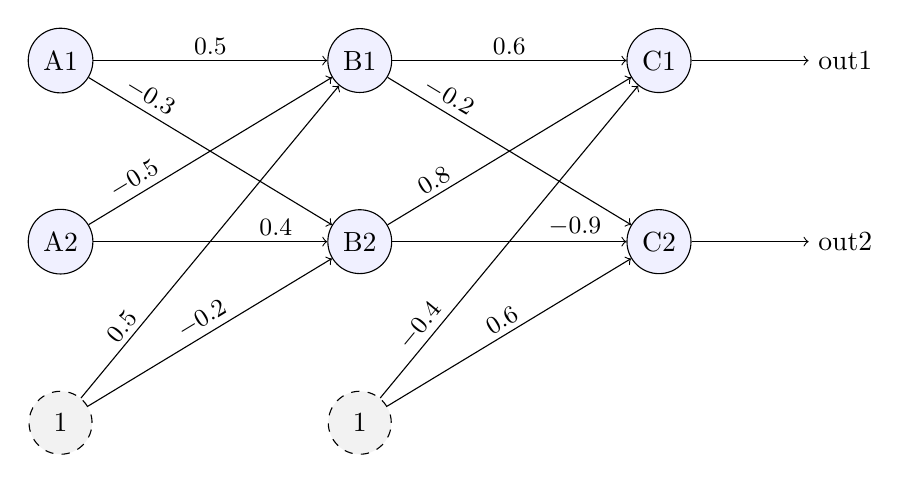
\begin{tikzpicture}[x=3.8cm,y=2.3cm,n/.style={circle,draw,minimum size=8mm,fill=blue!6},
  bn/.style={circle,draw,dashed,minimum size=8mm,fill=gray!10},
  w/.style={font=\small,fill=white,inner sep=1pt,sloped,above=1pt}]
\node[n] (A1) at (0,2) {A1}; \node[n] (A2) at (0,1) {A2}; \node[bn] (A0) at (0,0) {1};
\node[n] (B1) at (1,2) {B1}; \node[n] (B2) at (1,1) {B2}; \node[bn] (B0) at (1,0) {1};
\node[n] (C1) at (2,2) {C1}; \node[n] (C2) at (2,1) {C2};
% each weight is written near the start of its connection
\draw[->] (A1) -- node[w,pos=0.5] {0.5} (B1);
\draw[->] (A1) -- node[w,pos=0.22] {$-0.3$} (B2);
\draw[->] (A2) -- node[w,pos=0.22] {$-0.5$} (B1);
\draw[->] (A2) -- node[w,pos=0.78] {0.4} (B2);
\draw[->] (A0) -- node[w,pos=0.2] {0.5} (B1);
\draw[->] (A0) -- node[w,pos=0.5] {$-0.2$} (B2);
\draw[->] (B1) -- node[w,pos=0.5] {0.6} (C1);
\draw[->] (B1) -- node[w,pos=0.22] {$-0.2$} (C2);
\draw[->] (B2) -- node[w,pos=0.22] {0.8} (C1);
\draw[->] (B2) -- node[w,pos=0.78] {$-0.9$} (C2);
\draw[->] (B0) -- node[w,pos=0.2] {$-0.4$} (C1);
\draw[->] (B0) -- node[w,pos=0.5] {0.6} (C2);
\draw[->] (C1) -- ++(0.5,0) node[right] {out1}; \draw[->] (C2) -- ++(0.5,0) node[right] {out2};
\end{tikzpicture}
\end{center}
\prompt{Show the forward pass, in matrix form, of the record with Feature1 $= 4$ and Feature2 $= 2$. How would
this network classify the record (Class A or Class B)?}
\answerbox{10}
\begin{solution}
From the diagram:
\[
\bm{W}^{(1)} = \begin{pmatrix} 0.5 & -0.5 \\ -0.3 & 0.4 \end{pmatrix}, \quad
\bm{b}^{(1)} = \begin{pmatrix} 0.5 \\ -0.2 \end{pmatrix}, \quad
\bm{W}^{(2)} = \begin{pmatrix} 0.6 & 0.8 \\ -0.2 & -0.9 \end{pmatrix}, \quad
\bm{b}^{(2)} = \begin{pmatrix} -0.4 \\ 0.6 \end{pmatrix}.
\]
\[
\bm{z}_B = \bm{W}^{(1)} \bm{x} + \bm{b}^{(1)}
= \begin{pmatrix} 0.5 \cdot 4 - 0.5 \cdot 2 + 0.5 \\ -0.3 \cdot 4 + 0.4 \cdot 2 - 0.2 \end{pmatrix}
= \begin{pmatrix} 1.5 \\ -0.6 \end{pmatrix}, \quad
\bm{B} = \operatorname{ReLU}(\bm{z}_B) = \begin{pmatrix} 1.5 \\ 0 \end{pmatrix}
\]
\[
\bm{C} = \bm{W}^{(2)} \bm{B} + \bm{b}^{(2)}
= \begin{pmatrix} 0.6 \cdot 1.5 + 0.8 \cdot 0 - 0.4 \\ -0.2 \cdot 1.5 - 0.9 \cdot 0 + 0.6 \end{pmatrix}
= \begin{pmatrix} 0.5 \\ 0.3 \end{pmatrix}
\]
out1 $= 0.5 >$ out2 $= 0.3$: the network predicts Class A. (Forgetting the ReLU, and using
$B_2 = -0.6$, gives out1 $= 0.02$ and out2 $= 0.84$, the wrong class.)
\end{solution}

\newpage
\part[14] The network below has one hidden layer and one output, and will be trained for classification with log loss (cross-entropy loss). A record with inputs $A_1 = 2$,
$A_2 = 1$ and label $y = 1$ is passed in.
\begin{center}
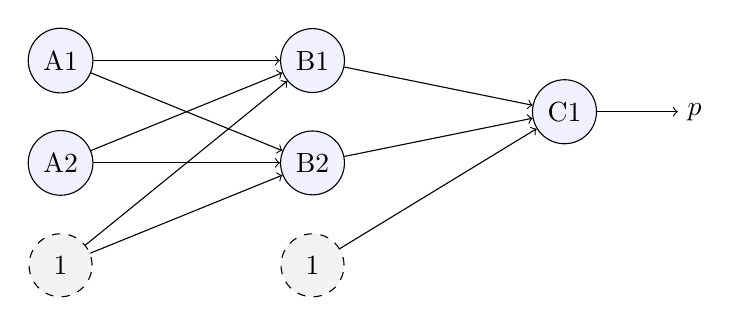
\begin{tikzpicture}[x=3.2cm,y=1.3cm,n/.style={circle,draw,minimum size=8mm,fill=blue!6},
  bn/.style={circle,draw,dashed,minimum size=8mm,fill=gray!10}]
\node[n] (A1) at (0,2) {A1}; \node[n] (A2) at (0,1) {A2}; \node[bn] (A0) at (0,0) {1};
\node[n] (B1) at (1,2) {B1}; \node[n] (B2) at (1,1) {B2}; \node[bn] (B0) at (1,0) {1};
\node[n] (C1) at (2,1.5) {C1};
\foreach \a in {A1,A2,A0} \foreach \b in {B1,B2} \draw[->] (\a) -- (\b);
\foreach \a in {B1,B2,B0} \draw[->] (\a) -- (C1);
\draw[->] (C1) -- ++(0.45,0) node[right] {$p$};
\end{tikzpicture}
\end{center}
\begin{center}
\begin{tabular}{|l|l|l|}
\hline
\rowcolor{headgray} activation function & function & derivative \\ \hline
B layer: sigmoid & $f(z) = 1/(1 + e^{-z})$ & $f(z)\,(1 - f(z))$ \\ \hline
C layer: sigmoid & $p = C_1 = 1/(1 + e^{-z_C})$ & (see the loss) \\ \hline
loss: cross-entropy & $\mathcal{L} = -y \log p - (1 - y) \log(1 - p)$ & $\partial \mathcal{L}/\partial z_C = p - y$ \\ \hline
\end{tabular}
\end{center}
Here $z_C$ is C1's input sum, and $p$ is the predicted probability that $y = 1$. The weights during the forward propagation are
\[
\bm{W}^{(1)} = \begin{pmatrix} 0.5 & -1.0 \\ 1.5 & 0.5 \end{pmatrix},\quad
\bm{b}^{(1)} = \begin{pmatrix} 0.5 \\ -1.0 \end{pmatrix},\qquad
\bm{W}^{(2)} = \begin{pmatrix} 1.0 & -2.0 \end{pmatrix},\quad b^{(2)} = 0.5 .
\]
You do not need to forward propagate. The node activations (output values) during the forward propagation are
\begin{center}
\begin{tabular}{|l|l|l|}
\hline
\rowcolor{headgray} A layer & B layer & C layer \\ \hline
$A_1 = 2$ & $B_1 = 0.62$ & $C_1 = p = 0.33$ \\ \hline
$A_2 = 1$ & $B_2 = 0.92$ & \\ \hline
\end{tabular}
\end{center}
Use a learning rate of 1. Compute every derivative with the weights above, the ones used in the
forward propagation.
\begin{subparts}
\subpart \prompt{Adjust $W^{(2)}_{11}$, the weight from B1 to C1.}
\answerbox[\thepartno(\thesubpart)]{5}
\ifprintanswers\else\newpage\fi   % keep (b) and its answer box together on the test
\subpart \prompt{Adjust $W^{(1)}_{11}$, the weight from A1 to B1.}
\answerbox[\thepartno(\thesubpart)]{10}
\end{subparts}
\begin{solution}
(a) The error at the output is $\partial \mathcal{L}/\partial z_C = p - y = 0.33 - 1 = -0.67$. Since
$z_C = W^{(2)}_{11} B_1 + W^{(2)}_{12} B_2 + b^{(2)}$, $\partial z_C/\partial W^{(2)}_{11} = B_1 = 0.62$, so
\[
\frac{\partial \mathcal{L}}{\partial W^{(2)}_{11}} = -0.67 \cdot 0.62 = -0.415, \qquad
W^{(2)}_{11} \leftarrow 1.0 - 1 \cdot (-0.415) = 1.415 .
\]
(b) The path is $W^{(1)}_{11} \to z_{B_1} \to B_1 \to z_C \to \mathcal{L}$, where $z_{B_1}$ is B1's input sum.
Reuse $-0.67$ from (a), with the old weight $W^{(2)}_{11} = 1.0$:
\[
\frac{\partial \mathcal{L}}{\partial B_1} = -0.67 \cdot 1.0 = -0.67, \qquad
\frac{\partial \mathcal{L}}{\partial z_{B_1}} = -0.67 \cdot B_1 (1 - B_1) = -0.67 \cdot 0.62 \cdot 0.38 = -0.158,
\]
\[
\frac{\partial \mathcal{L}}{\partial W^{(1)}_{11}} = -0.158 \cdot A_1 = -0.158 \cdot 2 = -0.316, \qquad
W^{(1)}_{11} \leftarrow 0.5 - 1 \cdot (-0.316) = 0.816 .
\]
(With unrounded node values the updates are 1.419 and 0.817; accept either.)
\end{solution}

\ifprintanswers\else\newpage\fi   % the short answers on one page of the test
\part Short answers (8 points in all).
\begin{subparts}
\subpart[3] \prompt{You train the same network twice with different learning rates and plot the training
loss after each epoch. In run 1 the loss jumps up and down and ends higher than it started. In run 2
it goes down steadily, but very slowly. For each run, is the learning rate too large or too small?
Why?}
\answerbox[\thepartno(\thesubpart)]{5}
\begin{solution}
Run 1: too large. Each step overshoots the minimum, so the loss bounces around and can grow.
Run 2: too small. Each step moves the weights only a little, so the loss falls slowly.
\end{solution}
\subpart[2] \prompt{A network classifies images into 3 classes. Why put a softmax on the three outputs
instead of a separate sigmoid on each?}
\answerbox[\thepartno(\thesubpart)]{4}
\begin{solution}
The softmax outputs are positive and add up to 1, so they are one probability distribution over the
3 classes. Separate sigmoids each give a number between 0 and 1, but they need not add up to 1 (all
three could be 0.9).
\end{solution}
\subpart[3] \prompt{A training set has 1,000 records. In one gradient-descent step, every weight in the
network is updated once. How many steps does training take in 5 epochs (number of passes through the
data) with (i) batch gradient descent, (ii) stochastic gradient descent (one record per step), and
(iii) mini-batches of 50 records?}
\answerbox[\thepartno(\thesubpart)]{4}
\begin{solution}
(i) One step per epoch: $5$. \quad (ii) $1{,}000$ steps per epoch: $5{,}000$. \quad
(iii) $1{,}000 / 50 = 20$ steps per epoch: $100$.
\end{solution}
\end{subparts}
\end{parts}

% ===================================================================== 5
\newpage
\titledquestion{Ensemble methods (10 points)}
\begin{parts}
\part[5] An SVM can only separate two classes. A clinic wants to classify chest X-rays into 4 classes:
normal, pneumonia, COVID and tuberculosis.
\begin{subparts}
\subpart \prompt{With one-vs-rest partitions, how many SVMs do you train, and what labels does each one
see?}
\subpart \prompt{How is a new X-ray classified?}
\subpart \prompt{With one-vs-one partitions, how many SVMs do you train?}
\end{subparts}
\answerbox{8}
\begin{solution}
(a) 4 SVMs, one per class. Each sees ``this class'' against ``the other three''.
(b) Each SVM predicts its side, and every class on the predicted side gets one vote; the class with the
most votes wins. (Also accept: pick the class whose SVM gives the largest $f(\bm{x})$.)
(c) One SVM for every pair of classes: $4 \cdot 3 / 2 = 6$.
\end{solution}

\part[3] \prompt{An ensemble of 25 classifiers is built, but each base classifier has error rate 0.6.
What happens to the error of the majority vote, compared with a single classifier? Why?}
\answerbox{5}
\begin{solution}
The ensemble is worse than a single classifier: with independent errors, the majority vote is wrong
whenever more than half of the classifiers are wrong, and with error 0.6 that happens most of the time
(about 0.85). A majority vote only helps when each base classifier is better than random guessing.
\end{solution}

\newpage
\part[2] \prompt{Random forests consider only a random subset of the features at each split. Why does
this help the ensemble?}
\answerbox{6}
\begin{solution}
It makes the trees less alike. Without it, every tree would split on the same strong features and make
similar mistakes; with random subsets the trees are more diverse, so their errors are less correlated
and the vote cancels more of them.
\end{solution}
\end{parts}

\end{questions}
\end{document}
"
\documentclass[11pt,addpoints]{exam}
\ifdefined\withsolutions \printanswers \fi
\usepackage{cs363m_exam}
\usepackage{pgfplots}
\pgfplotsset{compat=1.18}
\usepgfplotslibrary{groupplots}
% two options to circle: \pick{first}{second}{1 or 2}. The solutions circle the right one; the test
% draws the same frames invisibly, so the layout does not move.
\newcommand{\opt}[2]{% #2 is 1 for the right answer
  \def\optcolor{none}%
  \ifprintanswers\ifnum#2=1 \def\optcolor{red!70!black}\fi\fi
  \tikz[baseline=(o.base)]\node[inner sep=4pt,rounded corners=7pt,draw=\optcolor,very thick](o){#1};}
\newlength{\optw}\setlength{\optw}{3.6cm}   % each option sits in a column this wide
\newcommand{\pick}[3]{\hfill
  \makebox[\optw]{\ifnum#3=1 \opt{#1}{1}\else\opt{#1}{0}\fi}%
  \makebox[\optw]{\ifnum#3=2 \opt{#2}{1}\else\opt{#2}{0}\fi}}

\begin{document}
\ifprintanswers\examtitlepage{Midterm exam \textperiodcentered{} solutions}\else\examtitlepage{Midterm exam}\fi

\begin{questions}

% ===================================================================== 1
\titledquestion{Evaluating classifiers (20 points)}
A university wants to use an AI-text detector to check student essays. To test it, the detector is
run on 400 essays whose authorship is known: 60 were written with AI and 340 by students. Of the
400 essays, the detector flags 50 as written with AI. Of these 50 flagged essays, 45 really were
written with AI. Treat ``written with AI'' as the positive class.

\begin{parts}
\part[4] \prompt{Write down the confusion matrix.}
\ifprintanswers\else
\par\vspace{6pt}\noindent{\color{lbl}\textbf{Answer \thepartno}}
\begin{center}
\begin{tabular}{l|p{3cm}|p{3cm}|}
\multicolumn{1}{l}{} & \multicolumn{1}{c}{flagged} & \multicolumn{1}{c}{not flagged} \\
\cline{2-3}
written with AI & \rule[-0.45cm]{0pt}{1.2cm} & \\
\cline{2-3}
written by students & \rule[-0.45cm]{0pt}{1.2cm} & \\
\cline{2-3}
\end{tabular}
\end{center}
\fi
\begin{solution}
60 AI-written essays and 340 human-written essays.
\begin{center}
\begin{tabular}{|l|c|c|}
\hline
\rowcolor{headgray} & flagged & not flagged \\ \hline
written with AI & TP $= 45$ & FN $= 15$ \\ \hline
written by students & FP $= 5$  & TN $= 335$ \\ \hline
\end{tabular}
\end{center}
\end{solution}

\part[2] \prompt{What are precision and recall for this detector?}
\answerbox{5}
\begin{solution}
Precision $= 45/50 = 0.90$. \quad Recall $= 45/60 = 0.75$.
\end{solution}

\part[2] \prompt{Do we care more about improving precision or recall for this problem, and why?}
\answerbox{5}
\begin{solution}
Precision. A false positive accuses an innocent student of cheating; a missed AI essay (false
negative) is a smaller harm. A flag should almost always be right before anyone acts on it.
\end{solution}

\uplevel{The detector also gives each essay a score between 0 and 1; a higher score means ``more
likely written with AI''. Here are 8 essays, 4 written with AI and 4 by students:
\begin{center}
\begin{tabular}{|l|c|c|c|c|c|c|c|c|}
\hline
\rowcolor{headgray} essay            & 1 & 2 & 3 & 4 & 5 & 6 & 7 & 8 \\ \hline
score            & 0.95 & 0.85 & 0.70 & 0.60 & 0.50 & 0.40 & 0.30 & 0.10 \\ \hline
written with AI? & yes & yes & no & yes & no & yes & no & no \\ \hline
\end{tabular}
\end{center}
We say the detector flags an essay as AI-written if its score is over $t$.}

\part[10] \prompt{The ROC curve starts at $(\mathrm{FPR}, \mathrm{TPR}) = (0, 0)$, when $t$ is above every
score. Lower $t$ past one essay at a time. What are the next three points on the curve?}
\answerbox{8}
\begin{solution}
As $t$ passes each essay, from the highest score down, an AI essay moves the point up by
$1/4 = 0.25$ and a human essay moves it right by $0.25$. Essays 1 and 2 are AI-written and essay 3
is not, so the next three points are
\[
(0,\ 0.25), \quad (0,\ 0.5), \quad (0.25,\ 0.5).
\]
\end{solution}

\part[2] \prompt{Another detector has an AUC of 0.3 on the test essays. What does that tell you, and
what simple change would improve it?}
\answerbox{5}
\begin{solution}
It is worse than random guessing (AUC 0.5): it tends to give human-written essays higher scores than
AI-written ones. Flip it: use $1 - \text{score}$ (equivalently, flag the essays with low scores).
That reverses the order of the essays, so the AUC becomes $1 - 0.3 = 0.7$.
\end{solution}
\end{parts}

% ===================================================================== 2
\newpage
\titledquestion{Support vector machines (20 points)}
\begin{parts}
\part[10] A soft-margin SVM returned $\bm{w} = (6, 8)$, $b = -20$.
\begin{center}
\begin{tabular}{|l|c|c|c|}
\hline
\rowcolor{headgray} point  & C & D & E \\ \hline
$x_1$  & 1.5 & 1.25 & 3 \\ \hline
$x_2$  & 1.5 & 1.5 & 0.5 \\ \hline
label  & $+$ & $-$ & $-$ \\ \hline
\end{tabular}
\end{center}
\begin{subparts}
\subpart \prompt{Compute $f(\bm{x})$ and the predicted class of each point.}
\subpart \prompt{What is the width of the margin?}
\subpart \prompt{Which points are on the margin? Which points are inside the margin? Which points are
misclassified?}
\end{subparts}
\answerbox{16}
\begin{solution}
$f(\bm{x}) = 6x_1 + 8x_2 - 20$ and $\|\bm{w}\| = \sqrt{6^2 + 8^2} = 10$.
\begin{center}
\begin{tabular}{|l|c|c|c|}
\hline
\rowcolor{headgray} point & C & D & E \\ \hline
$f(\bm{x})$                       & $1$   & $-0.5$ & $2$ \\ \hline
predicted class                   & $+$   & $-$    & $+$ \\ \hline
$y\,f(\bm{x})$                    & $1$   & $0.5$  & $-2$ \\ \hline
\end{tabular}
\end{center}
(b) Margin width $= 2/\|\bm{w}\| = 2/10 = 0.2$.

(c) On the margin: C ($y\,f = 1$). Inside the margin: D ($0 < y\,f = 0.5 < 1$), still correctly
classified. Misclassified: E (label $-$, predicted $+$; $y\,f = -2$).
\end{solution}

\part[4] The soft-margin SVM solves
\[
\min_{\bm{w},\, b,\, \bm{\xi}} \ \tfrac12 \|\bm{w}\|^2 + C \sum_i \xi_i
\quad \text{subject to} \quad y_i(\bm{w} \cdot \bm{x}_i + b) \ge 1 - \xi_i,\ \ \xi_i \ge 0 .
\]
\begin{subparts}
\subpart \prompt{What does the slack $\xi_i$ measure, and why do we need it?}
\subpart \prompt{Where does a training point lie, relative to the margin and the decision boundary, if
$\xi_i > 1$?}
\end{subparts}
\answerbox{8}
\begin{solution}
(a) $\xi_i$ measures how far point $i$ falls short of being on its correct side, outside the margin.
Without slack, the constraints $y_i(\bm{w} \cdot \bm{x}_i + b) \ge 1$ have no solution when the
classes overlap; slack lets some points violate the margin, at a cost $C\xi_i$ each.

(b) On the wrong side of the decision boundary: misclassified. (At the solution
$\xi_i = \max(0,\, 1 - y_i f(\bm{x}_i))$, so $\xi_i > 1$ means $y_i f(\bm{x}_i) < 0$.)
\end{solution}

\part[4] Two soft-margin SVMs are trained on the same data, one with $C = 0.01$ and one with
$C = 100$.
For (a)--(c), circle one answer.
\begin{subparts}
\subpart \prompt{Which has the wider margin?} \pick{$C = 0.01$}{$C = 100$}{1}
\subpart \prompt{Which has more support vectors?} \pick{$C = 0.01$}{$C = 100$}{1}
\subpart \prompt{Which is more likely to overfit?} \pick{$C = 0.01$}{$C = 100$}{2}
\subpart \prompt{How would you choose $C$ in practice, and why?}
\end{subparts}
\answerbox[\thepartno(d)]{4}
\begin{solution}
(a) $C = 0.01$: slack is cheap, so the SVM accepts many points inside the margin in exchange for a
wider one.
(b) $C = 0.01$: with a wider margin, more points fall on or inside it, and all of them are support
vectors.
(c) $C = 100$: violations are expensive, so the margin narrows to fit individual training points.
(d) $C$ is a hyperparameter: try several values and pick the one with the best accuracy on
validation data (or by cross-validation). Training accuracy cannot choose it, because a larger $C$
always fits the training data at least as well; only held-out data shows which $C$ generalizes.
\end{solution}

\ifprintanswers\else\newpage\fi   % keep 2.4 together on the test
\part[2] \prompt{You remove a training point that is not a support vector and retrain the SVM. What
changes? Why?}
\answerbox{5}
\begin{solution}
Nothing. The solution depends only on the support vectors; a point outside the margin does not
affect $\bm{w}$ or $b$.
\end{solution}
\end{parts}

% ===================================================================== 3
\newpage
\titledquestion{Nonlinear regression (20 points)}
\begin{parts}
\part[4] kNN regression is trained on six points:
\begin{center}
\begin{tabular}{|l|c|c|c|c|c|c|}
\hline
$x$ & 1 & 2 & 4 & 5 & 7 & 8 \\ \hline
$y$ & 3 & 6 & 4 & 8 & 10 & 12 \\ \hline
\end{tabular}
\end{center}
\prompt{Predict $y$ at $x = 4.4$ using (a) $k = 1$ and (b) $k = 3$.}
\answerbox{3}
\begin{solution}
(a) The nearest point is $x = 4$, so the prediction is $4$.
(b) The three nearest points are $x = 4, 5, 2$ (distances $0.4, 0.6, 2.4$), so the prediction is
$(4 + 8 + 6)/3 = 6$.
\end{solution}

\part[6] \prompt{For each model, name a hyperparameter that controls how closely the model fits the
training data. Does increasing it make overfitting more likely or less likely? Fill in the table.}
\begin{center}
\renewcommand{\arraystretch}{1.25}
\ifprintanswers
\begin{tabular}{|>{\raggedright\arraybackslash}p{3.3cm}|>{\raggedright\arraybackslash}p{5.2cm}|>{\raggedright\arraybackslash}p{4.2cm}|}
\hline
\rowcolor{headgray} \textbf{Model} & \textbf{Hyperparameter} & \textbf{Increasing it $\to$}\newline \textbf{MORE / LESS overfitting} \\ \hline
Regression tree & maximum depth & MORE \\ \hline
kNN regression & number of neighbours $k$ & LESS \\ \hline
SVR & $C$ & MORE \\ \hline
\end{tabular}
\else
\begin{tabular}{|>{\raggedright\arraybackslash}p{3.3cm}|>{\raggedright\arraybackslash}p{5.2cm}|>{\raggedright\arraybackslash}p{4.2cm}|}
\hline
\rowcolor{headgray} \textbf{Model} & \textbf{Hyperparameter} & \textbf{Increasing it $\to$}\newline \textbf{MORE / LESS overfitting} \\ \hline
Regression tree \rule[-0.5cm]{0pt}{1.3cm} & & \\ \hline
kNN regression \rule[-0.5cm]{0pt}{1.3cm} & & \\ \hline
SVR \rule[-0.5cm]{0pt}{1.3cm} & & \\ \hline
\end{tabular}
\fi
\end{center}
\begin{solution}
Other correct answers: for the tree, the minimum number of points needed to split (increasing it:
LESS); for SVR, $\varepsilon$ (increasing it: LESS). The direction must match the hyperparameter named.
\end{solution}

\newpage
\part[5] \prompt{The figure shows three models fitted to the same data. Which panel shows a regression
tree, which shows kNN with $k = 1$, and which shows SVR with a kernel? Explain each.}
\begin{center}
% Question 3.3 of the exam: three fits of the same data (data from ../make_figure.py)
\begin{tikzpicture}
\begin{groupplot}[group style={group size=3 by 1, horizontal sep=1.1cm},
    width=5.6cm, height=4.6cm, xmin=0, xmax=10, ymin=2.5, ymax=7, xtick={0,5,10}, ytick={3,5,7},
    xlabel={$x$}, ylabel={$y$}, ylabel style={yshift=-4pt}, title style={font=\bfseries}]
\nextgroupplot[title=A]
  \addplot[thick, blue!70!black] table {fig_data/svr.dat};
  \addplot[only marks, mark=*, mark size=1.6pt] table {fig_data/points.dat};
\nextgroupplot[title=B]
  \addplot[thick, blue!70!black] table {fig_data/tree.dat};
  \addplot[only marks, mark=*, mark size=1.6pt] table {fig_data/points.dat};
\nextgroupplot[title=C]
  \addplot[thick, blue!70!black] table {fig_data/knn.dat};
  \addplot[only marks, mark=*, mark size=1.6pt] table {fig_data/points.dat};
\end{groupplot}
\end{tikzpicture}

\end{center}
\answerbox{6}
\begin{solution}
A is SVR with a kernel: a smooth curve. B is the regression tree: a few wide flat steps, one for
each leaf, which predicts the average $y$ of its points. C is kNN with $k = 1$: a narrow step for
every training point, passing through every point.
\end{solution}

\part[5] \prompt{Suppose you use kNN to predict house prices from floor area (500 to 5,000 square feet) and number
of bedrooms (1 to 6). Why might kNN do badly on these raw features? What would you do?}
\answerbox{6}
\begin{solution}
Distances are dominated by floor area: a difference of one bedroom counts as much as one square
foot, so the nearest houses match on area and almost ignore bedrooms. Standardize each feature
(subtract its mean, divide by its standard deviation) before computing distances.
\end{solution}
\end{parts}

% ===================================================================== 4
\newpage
\titledquestion{Neural networks (30 points)}
In this question, row $j$ of a weight matrix $\bm{W}^{(l)}$ holds the weights into node $j$ of layer
$l$: $W^{(l)}_{ji}$ is the weight from node $i$ of the previous layer to node $j$. The bias of node
$j$ is $b^{(l)}_j$, the weight on the input that is always 1.

\begin{parts}
\part[8] In the network below, out1 represents Class A and out2 represents Class B. The hidden nodes
B1 and B2 use the ReLU activation, $\operatorname{ReLU}(z) = \max(0, z)$. The output nodes C1 and C2
have no activation: each outputs its weighted sum. The network predicts the class whose output is
larger.
\begin{center}
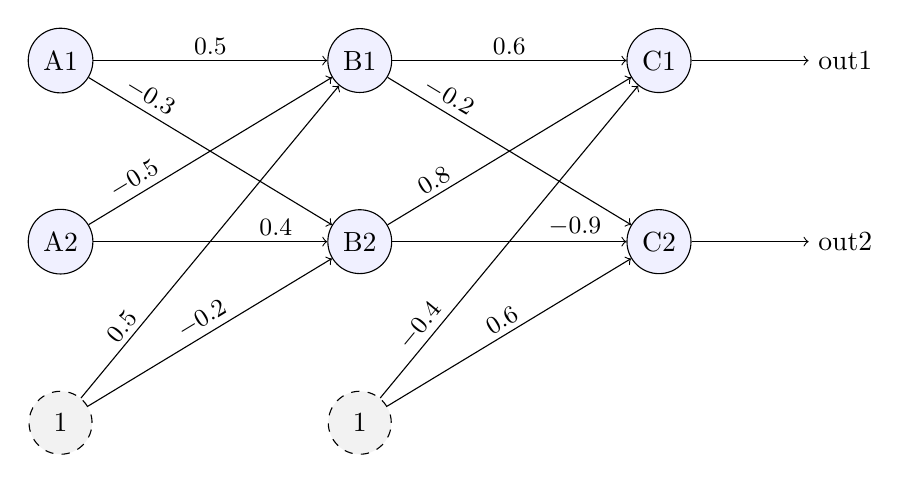
\begin{tikzpicture}[x=3.8cm,y=2.3cm,n/.style={circle,draw,minimum size=8mm,fill=blue!6},
  bn/.style={circle,draw,dashed,minimum size=8mm,fill=gray!10},
  w/.style={font=\small,fill=white,inner sep=1pt,sloped,above=1pt}]
\node[n] (A1) at (0,2) {A1}; \node[n] (A2) at (0,1) {A2}; \node[bn] (A0) at (0,0) {1};
\node[n] (B1) at (1,2) {B1}; \node[n] (B2) at (1,1) {B2}; \node[bn] (B0) at (1,0) {1};
\node[n] (C1) at (2,2) {C1}; \node[n] (C2) at (2,1) {C2};
% each weight is written near the start of its connection
\draw[->] (A1) -- node[w,pos=0.5] {0.5} (B1);
\draw[->] (A1) -- node[w,pos=0.22] {$-0.3$} (B2);
\draw[->] (A2) -- node[w,pos=0.22] {$-0.5$} (B1);
\draw[->] (A2) -- node[w,pos=0.78] {0.4} (B2);
\draw[->] (A0) -- node[w,pos=0.2] {0.5} (B1);
\draw[->] (A0) -- node[w,pos=0.5] {$-0.2$} (B2);
\draw[->] (B1) -- node[w,pos=0.5] {0.6} (C1);
\draw[->] (B1) -- node[w,pos=0.22] {$-0.2$} (C2);
\draw[->] (B2) -- node[w,pos=0.22] {0.8} (C1);
\draw[->] (B2) -- node[w,pos=0.78] {$-0.9$} (C2);
\draw[->] (B0) -- node[w,pos=0.2] {$-0.4$} (C1);
\draw[->] (B0) -- node[w,pos=0.5] {0.6} (C2);
\draw[->] (C1) -- ++(0.5,0) node[right] {out1}; \draw[->] (C2) -- ++(0.5,0) node[right] {out2};
\end{tikzpicture}
\end{center}
\prompt{Show the forward pass, in matrix form, of the record with Feature1 $= 4$ and Feature2 $= 2$. How would
this network classify the record (Class A or Class B)?}
\answerbox{10}
\begin{solution}
From the diagram:
\[
\bm{W}^{(1)} = \begin{pmatrix} 0.5 & -0.5 \\ -0.3 & 0.4 \end{pmatrix}, \quad
\bm{b}^{(1)} = \begin{pmatrix} 0.5 \\ -0.2 \end{pmatrix}, \quad
\bm{W}^{(2)} = \begin{pmatrix} 0.6 & 0.8 \\ -0.2 & -0.9 \end{pmatrix}, \quad
\bm{b}^{(2)} = \begin{pmatrix} -0.4 \\ 0.6 \end{pmatrix}.
\]
\[
\bm{z}_B = \bm{W}^{(1)} \bm{x} + \bm{b}^{(1)}
= \begin{pmatrix} 0.5 \cdot 4 - 0.5 \cdot 2 + 0.5 \\ -0.3 \cdot 4 + 0.4 \cdot 2 - 0.2 \end{pmatrix}
= \begin{pmatrix} 1.5 \\ -0.6 \end{pmatrix}, \quad
\bm{B} = \operatorname{ReLU}(\bm{z}_B) = \begin{pmatrix} 1.5 \\ 0 \end{pmatrix}
\]
\[
\bm{C} = \bm{W}^{(2)} \bm{B} + \bm{b}^{(2)}
= \begin{pmatrix} 0.6 \cdot 1.5 + 0.8 \cdot 0 - 0.4 \\ -0.2 \cdot 1.5 - 0.9 \cdot 0 + 0.6 \end{pmatrix}
= \begin{pmatrix} 0.5 \\ 0.3 \end{pmatrix}
\]
out1 $= 0.5 >$ out2 $= 0.3$: the network predicts Class A. (Forgetting the ReLU, and using
$B_2 = -0.6$, gives out1 $= 0.02$ and out2 $= 0.84$, the wrong class.)
\end{solution}

\newpage
\part[14] The network below has one hidden layer and one output, and will be trained for classification with log loss (cross-entropy loss). A record with inputs $A_1 = 2$,
$A_2 = 1$ and label $y = 1$ is passed in.
\begin{center}
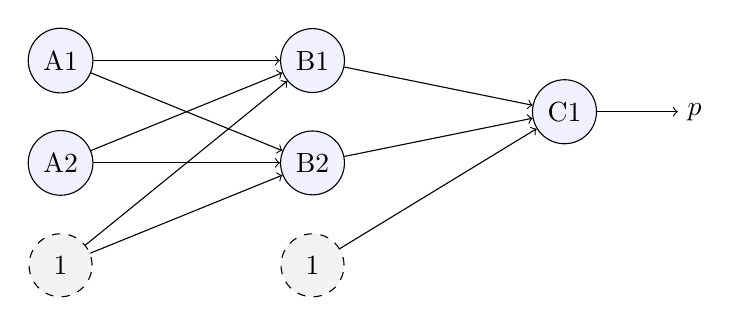
\begin{tikzpicture}[x=3.2cm,y=1.3cm,n/.style={circle,draw,minimum size=8mm,fill=blue!6},
  bn/.style={circle,draw,dashed,minimum size=8mm,fill=gray!10}]
\node[n] (A1) at (0,2) {A1}; \node[n] (A2) at (0,1) {A2}; \node[bn] (A0) at (0,0) {1};
\node[n] (B1) at (1,2) {B1}; \node[n] (B2) at (1,1) {B2}; \node[bn] (B0) at (1,0) {1};
\node[n] (C1) at (2,1.5) {C1};
\foreach \a in {A1,A2,A0} \foreach \b in {B1,B2} \draw[->] (\a) -- (\b);
\foreach \a in {B1,B2,B0} \draw[->] (\a) -- (C1);
\draw[->] (C1) -- ++(0.45,0) node[right] {$p$};
\end{tikzpicture}
\end{center}
\begin{center}
\begin{tabular}{|l|l|l|}
\hline
\rowcolor{headgray} activation function & function & derivative \\ \hline
B layer: sigmoid & $f(z) = 1/(1 + e^{-z})$ & $f(z)\,(1 - f(z))$ \\ \hline
C layer: sigmoid & $p = C_1 = 1/(1 + e^{-z_C})$ & (see the loss) \\ \hline
loss: cross-entropy & $\mathcal{L} = -y \log p - (1 - y) \log(1 - p)$ & $\partial \mathcal{L}/\partial z_C = p - y$ \\ \hline
\end{tabular}
\end{center}
Here $z_C$ is C1's input sum, and $p$ is the predicted probability that $y = 1$. The weights during the forward propagation are
\[
\bm{W}^{(1)} = \begin{pmatrix} 0.5 & -1.0 \\ 1.5 & 0.5 \end{pmatrix},\quad
\bm{b}^{(1)} = \begin{pmatrix} 0.5 \\ -1.0 \end{pmatrix},\qquad
\bm{W}^{(2)} = \begin{pmatrix} 1.0 & -2.0 \end{pmatrix},\quad b^{(2)} = 0.5 .
\]
You do not need to forward propagate. The node activations (output values) during the forward propagation are
\begin{center}
\begin{tabular}{|l|l|l|}
\hline
\rowcolor{headgray} A layer & B layer & C layer \\ \hline
$A_1 = 2$ & $B_1 = 0.62$ & $C_1 = p = 0.33$ \\ \hline
$A_2 = 1$ & $B_2 = 0.92$ & \\ \hline
\end{tabular}
\end{center}
Use a learning rate of 1. Compute every derivative with the weights above, the ones used in the
forward propagation.
\begin{subparts}
\subpart \prompt{Adjust $W^{(2)}_{11}$, the weight from B1 to C1.}
\answerbox[\thepartno(\thesubpart)]{5}
\ifprintanswers\else\newpage\fi   % keep (b) and its answer box together on the test
\subpart \prompt{Adjust $W^{(1)}_{11}$, the weight from A1 to B1.}
\answerbox[\thepartno(\thesubpart)]{10}
\end{subparts}
\begin{solution}
(a) The error at the output is $\partial \mathcal{L}/\partial z_C = p - y = 0.33 - 1 = -0.67$. Since
$z_C = W^{(2)}_{11} B_1 + W^{(2)}_{12} B_2 + b^{(2)}$, $\partial z_C/\partial W^{(2)}_{11} = B_1 = 0.62$, so
\[
\frac{\partial \mathcal{L}}{\partial W^{(2)}_{11}} = -0.67 \cdot 0.62 = -0.415, \qquad
W^{(2)}_{11} \leftarrow 1.0 - 1 \cdot (-0.415) = 1.415 .
\]
(b) The path is $W^{(1)}_{11} \to z_{B_1} \to B_1 \to z_C \to \mathcal{L}$, where $z_{B_1}$ is B1's input sum.
Reuse $-0.67$ from (a), with the old weight $W^{(2)}_{11} = 1.0$:
\[
\frac{\partial \mathcal{L}}{\partial B_1} = -0.67 \cdot 1.0 = -0.67, \qquad
\frac{\partial \mathcal{L}}{\partial z_{B_1}} = -0.67 \cdot B_1 (1 - B_1) = -0.67 \cdot 0.62 \cdot 0.38 = -0.158,
\]
\[
\frac{\partial \mathcal{L}}{\partial W^{(1)}_{11}} = -0.158 \cdot A_1 = -0.158 \cdot 2 = -0.316, \qquad
W^{(1)}_{11} \leftarrow 0.5 - 1 \cdot (-0.316) = 0.816 .
\]
(With unrounded node values the updates are 1.419 and 0.817; accept either.)
\end{solution}

\ifprintanswers\else\newpage\fi   % the short answers on one page of the test
\part Short answers (8 points in all).
\begin{subparts}
\subpart[3] \prompt{You train the same network twice with different learning rates and plot the training
loss after each epoch. In run 1 the loss jumps up and down and ends higher than it started. In run 2
it goes down steadily, but very slowly. For each run, is the learning rate too large or too small?
Why?}
\answerbox[\thepartno(\thesubpart)]{5}
\begin{solution}
Run 1: too large. Each step overshoots the minimum, so the loss bounces around and can grow.
Run 2: too small. Each step moves the weights only a little, so the loss falls slowly.
\end{solution}
\subpart[2] \prompt{A network classifies images into 3 classes. Why put a softmax on the three outputs
instead of a separate sigmoid on each?}
\answerbox[\thepartno(\thesubpart)]{4}
\begin{solution}
The softmax outputs are positive and add up to 1, so they are one probability distribution over the
3 classes. Separate sigmoids each give a number between 0 and 1, but they need not add up to 1 (all
three could be 0.9).
\end{solution}
\subpart[3] \prompt{A training set has 1,000 records. In one gradient-descent step, every weight in the
network is updated once. How many steps does training take in 5 epochs (number of passes through the
data) with (i) batch gradient descent, (ii) stochastic gradient descent (one record per step), and
(iii) mini-batches of 50 records?}
\answerbox[\thepartno(\thesubpart)]{4}
\begin{solution}
(i) One step per epoch: $5$. \quad (ii) $1{,}000$ steps per epoch: $5{,}000$. \quad
(iii) $1{,}000 / 50 = 20$ steps per epoch: $100$.
\end{solution}
\end{subparts}
\end{parts}

% ===================================================================== 5
\newpage
\titledquestion{Ensemble methods (10 points)}
\begin{parts}
\part[5] An SVM can only separate two classes. A clinic wants to classify chest X-rays into 4 classes:
normal, pneumonia, COVID and tuberculosis.
\begin{subparts}
\subpart \prompt{With one-vs-rest partitions, how many SVMs do you train, and what labels does each one
see?}
\subpart \prompt{How is a new X-ray classified?}
\subpart \prompt{With one-vs-one partitions, how many SVMs do you train?}
\end{subparts}
\answerbox{8}
\begin{solution}
(a) 4 SVMs, one per class. Each sees ``this class'' against ``the other three''.
(b) Each SVM predicts its side, and every class on the predicted side gets one vote; the class with the
most votes wins. (Also accept: pick the class whose SVM gives the largest $f(\bm{x})$.)
(c) One SVM for every pair of classes: $4 \cdot 3 / 2 = 6$.
\end{solution}

\part[3] \prompt{An ensemble of 25 classifiers is built, but each base classifier has error rate 0.6.
What happens to the error of the majority vote, compared with a single classifier? Why?}
\answerbox{5}
\begin{solution}
The ensemble is worse than a single classifier: with independent errors, the majority vote is wrong
whenever more than half of the classifiers are wrong, and with error 0.6 that happens most of the time
(about 0.85). A majority vote only helps when each base classifier is better than random guessing.
\end{solution}

\newpage
\part[2] \prompt{Random forests consider only a random subset of the features at each split. Why does
this help the ensemble?}
\answerbox{6}
\begin{solution}
It makes the trees less alike. Without it, every tree would split on the same strong features and make
similar mistakes; with random subsets the trees are more diverse, so their errors are less correlated
and the vote cancels more of them.
\end{solution}
\end{parts}

\end{questions}
\end{document}
